

\chapter{Population Structure and Correlations Among Loci.}
\newthought{Individuals rarely mate completely at random}; your parents
weren't two Bilateria plucked at random from the tree of
life.
%JRI: what's up with the newthought formatting? new here and not used in similar sections
Even within species, there's often geographically-restricted
mating among individuals. Individuals tend to mate with individuals
from the same, or closely related sets of populations. This form of
non-random mating is called population structure and can have profound
effects on the distribution of genetic variation within and among
natural populations.

Populations can often differ in their allele frequencies, either due
to genetic drift or selection driving differentiation among
populations. In this chapter we'll talk through some ways to summarize and
visualize population genetic structure. Population differentiation is also a major driver of
correlations in allelic state among loci, and we'll start our
discussion of these correlations at the end of this chapter.
One reason for talking about population structure so early in the book is
that summarizing population structure is often a key initial stage in
population genomic analyses. Thus you'll often encounter summaries and visualizations of
population structure when we read research papers, so it's good to
have some understanding of what they represent.  

\subsection{Inbreeding as a summary of population structure.} \label{section:F_stats}
Our statements about inbreeding, and inbreeding coefficients, represent one natural
way to summarize population structure. In the previous chapter, we defined inbreeding as having parents that are more closely related to each other than two individuals drawn at random from some reference population. The question that naturally arises is: Which reference population should we use? While I might not look inbred in
comparison to allele frequencies in the United Kingdom (UK), where I am from, my
parents certainly are not two individuals drawn at random from the
world-wide population. If we estimated my inbreeding coefficient $F$ using allele frequencies
within the UK, it would
be close to zero, but would likely be larger if we used world-wide
frequencies. This is because there is a somewhat lower level of
expected heterozygosity within the UK than in the human population across the world as a whole.\\

Building on this idea of inbreeding coefficients estimated at various
levels, \citeauthor{Wright:43} developed a set of `F-statistics' (also called `fixation
indices') that formalize the idea of inbreeding with respect to different
levels of population structure \citep{Wright:43,Wright:49}. See Figure \ref{fig:FST_pig} for a schematic
diagram. Wright defined $F_{\mathrm{XY}}$ as the correlation between random
gametes, drawn from the same level $X$, relative to level $Y$. We will return
to why $F$-statistics are statements about correlations between alleles in just
a moment. One commonly used $F$-statistic is $\fis$, which is the inbreeding
coefficient between an individual ($I$) and the subpopulation ($S$). Consider a
single locus, where in a subpopulation ($S$) a fraction $H_I=f_{12}$ of
individuals are heterozygous.  In this subpopulation, let the frequency of
allele $A_1$ be $p_S$, such that the expected heterozygosity under random
mating is $H_S = 2 p_S (1 - p_S)$. We will write $\fis$ as
\begin{marginfigure}
\begin{center}
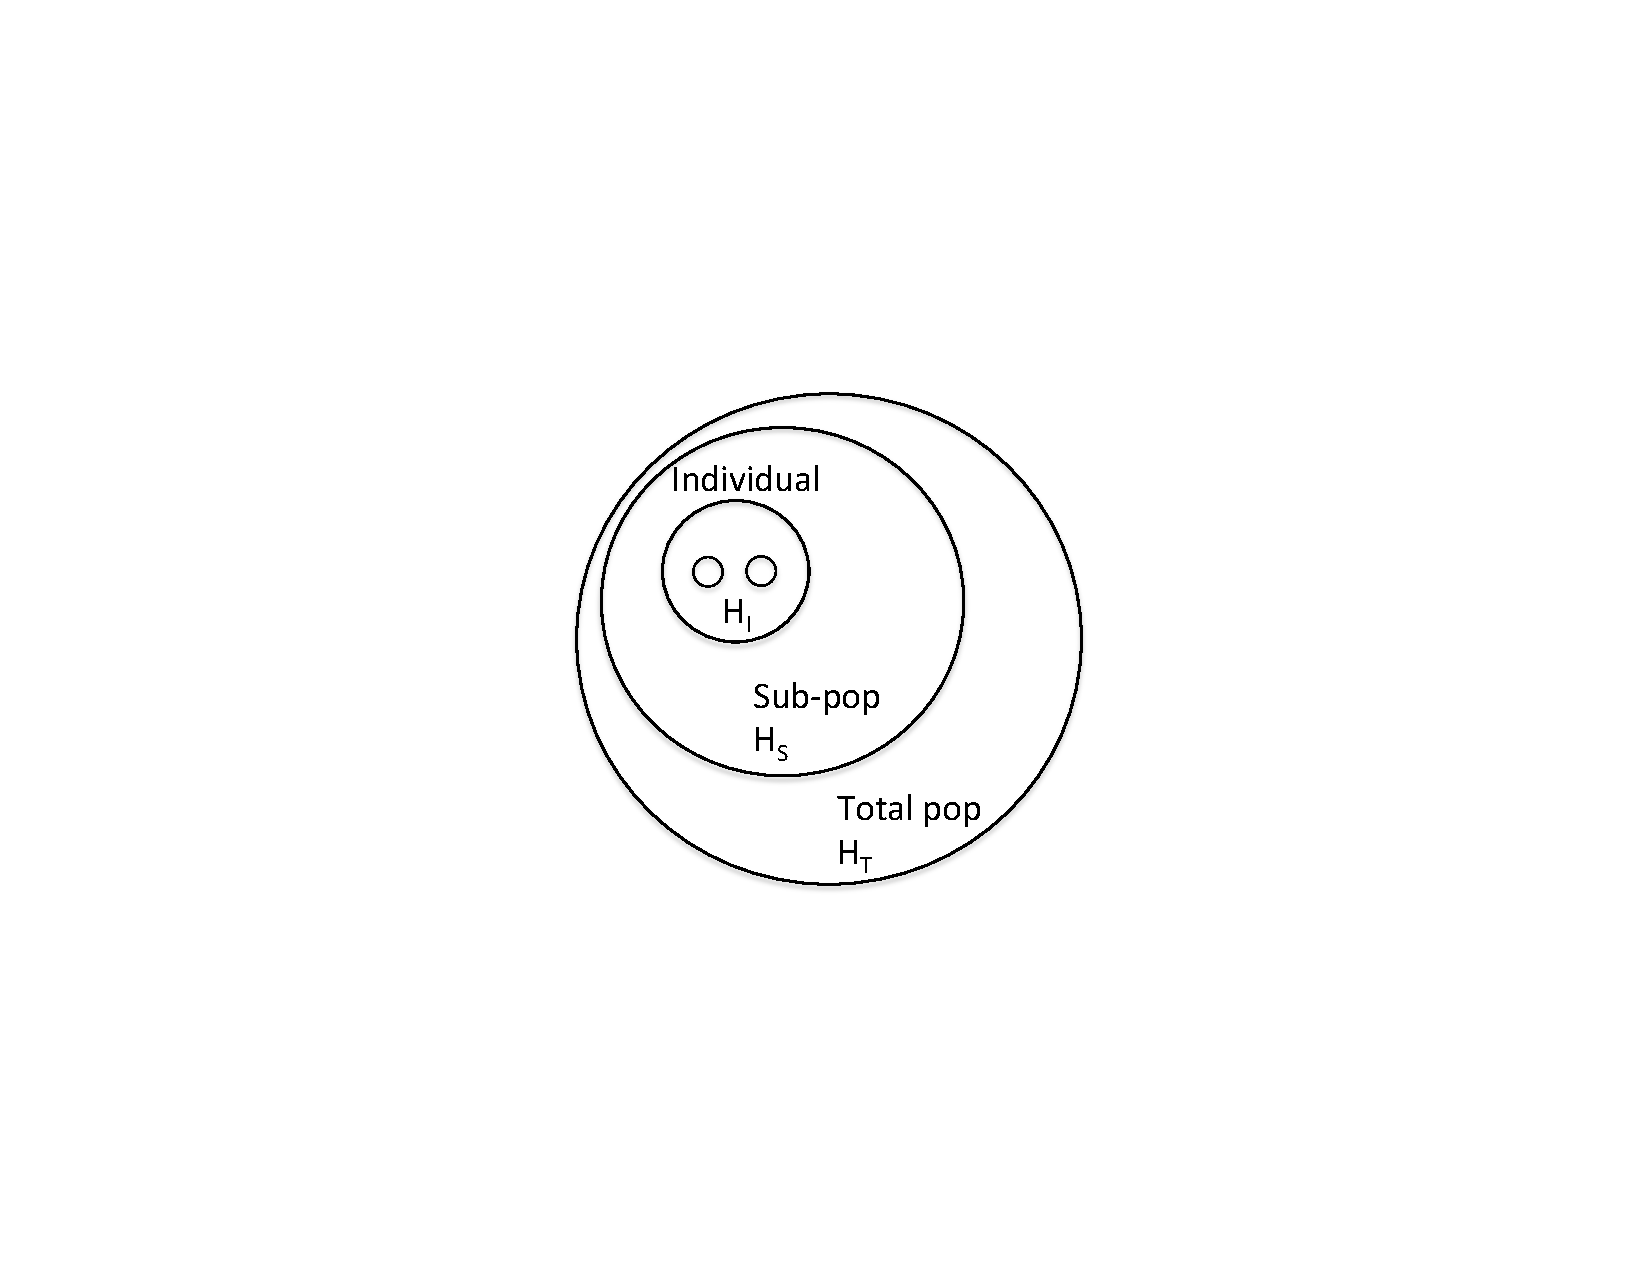
\includegraphics[width=\textwidth]{figures/Pop_struct/FST_hierarchy.pdf}  %
\end{center}
\caption{The hierarchical nature of F-statistics. The two dots within an individual represent the two
  alleles at a locus for an individual $I$. We can compare the heterozygosity in individuals ($H_I$), to that found
by randomly drawing alleles from the sub-population (S),
to that found in the total population (T). } \label{fig:FST_pig}
\end{marginfigure}
\begin{equation}
\fis = 1-\frac{H_I}{H_S}= 1-\frac{f_{12}}{2p_Sq_S},
\label{eqn:FIS}
\end{equation}
a direct analog of \eqn \ref{eqn:Fhat}. Hence, $\fis$ is the relative difference between observed and expected heterozygosity due to a deviation from random mating within the subpopulation. We could also compare the observed
heterozygosity in individuals ($H_I$) to that expected in the total
population, $H_T$. If the frequency of allele $A_1$ in the total
population is $p_T$, then we can write $\fit$ as
\begin{equation}
\fit =1-\frac{H_I}{H_T}= 1-\frac{f_{12}}{2p_Tq_T},
\label{eqn:FIT}
\end{equation}
which compares heterozygosity in individuals to that expected in the
total population. As a simple extension of this, we could imagine
comparing the expected heterozygosity in the subpopulation ($H_S$) to
that expected in the total population $H_T$, via $\fst$:
\begin{equation}
\fst = 1-\frac{H_S}{H_T}=1-\frac{2p_Sq_S}{2p_Tq_T} \label{eqn:FST}.
\end{equation}
 We can
relate the three $F$-statistics to each other as
\begin{equation}
(1-\fit) =\frac{H_I}{H_S} \frac{H_S}{H_T}=(1-\fis)(1-\fst).
\label{eqn:F_relationships}
\end{equation}
Hence, the reduction in heterozygosity within individuals compared to that expected
in the total population can be decomposed to the reduction in
heterozygosity of individuals compared to the subpopulation, and the reduction in
heterozygosity from the total population to that in the subpopulation.\\
%n, as we will seebelow, due to the Wahlund effect (to be added)

If we want a summary of
population structure across multiple subpopulations, we can average $H_I$
and/or $H_S$ across populations, and use a $p_T$ calculated by
averaging $p_S$ across subpopulations (or our samples from sub-populations). For example, the average $\fst$ across $K$ subpopulations (sampled with equal effort) is
\begin{equation}
	\fst = 1 - \frac{\bar{H}_{S}}{H_T},
\end{equation}
where $\bar{H}_S = \nicefrac{1}{K} \sum_{i = 1}^{K} H_{S}^{(i)}$, and
$H_{S}^{(i)} = 2 p_{i} q_{i}$ is the expected heterozygosity in subpopulation
$i$. It follows that the  average heterozygosity of the
sub-populations $\bar{H}_S  \leq
H_T$, and so $\fst \geq 0$ and $\fis \leq \fit$. This observation that the average
  heterozygosity of the sub-populations must be less than of equal to
  that of the total
  population is called the Wahlund effect. Furthermore, if we have multiple sites, we can replace $H_I$, $H_S$, and
$H_T$ with their averages across loci (as above).\sidenote[][-0.5cm]{Averaging heterozygosity across loci first, then calculating $\fst$, rather than calculating $\fst$ for each locus individually and then taking the average, has better statistical properties as statistical noise in the denominator is averaged out. }


As an example of comparing a genome-wide estimate of $F_{ST}$ to that
at individual loci we can look at some data from blue- and
golden-winged warblers ({\it Vermivora cyanoptera} and {\it
  V. chrysoptera} 1-2 \& 5-6 in Figure  \ref{fig:blue_golden_warblers}).
  \begin{marginfigure}[2.5cm]
\begin{center}
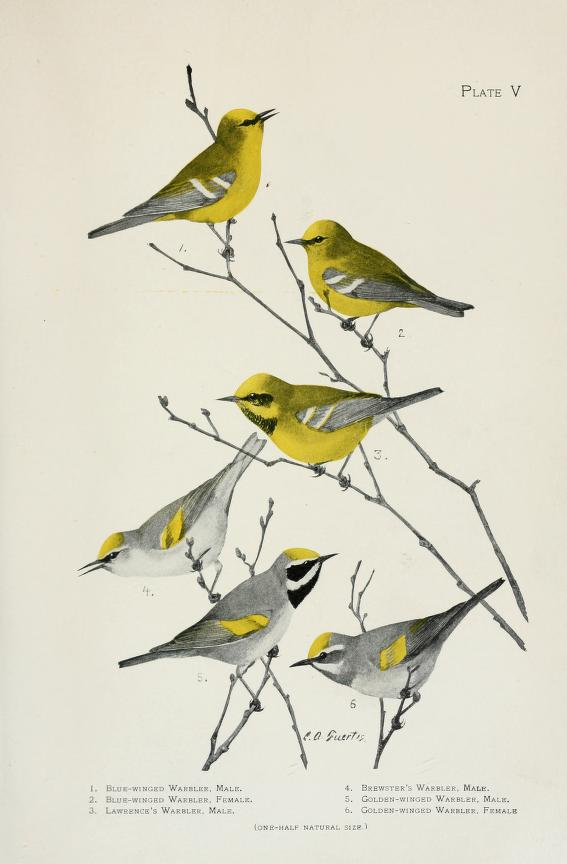
\includegraphics[width = \textwidth]{illustration_images/alleles_genotypes/blue_golden_winged_warblers/The_warblers_of_North_America_6309257188.jpg}  %[width= \marginwidth]
\end{center}
\caption{Blue-, golden-winged, and Lawrence's warblers ({\it Vermivora}). \BHLNC{The warblers of North America. Chapman, F.M. 1907.}{https://www.biodiversitylibrary.org/page/9165714\#page/101/mode/1up}{American Museum of Natural History Library}} \label{fig:blue_golden_warblers}
\end{marginfigure}
These two species are spread across eastern
Northern America, with the golden-winged warbler having a smaller, more
northernly range. They're quite different in terms of plumage, but
have long been known to have similar songs and ecologies. The two species
hybridize readily in the wild; in fact two other previously-recognized species, Brewster's
and Lawrence's warbler (4 \& 3 in \ref{fig:blue_golden_warblers}), are
actually found to just be hybrids between theses two
species. \graham{Add ref to Bateson book }
% https://twitter.com/WTF_R_species/status/1046586267167854592 & https://twitter.com/davetoews/status/1046599444878282752
The golden-winged warbler is listed as `threatened' under the Canadian
endangered species act as its habitat is under pressure from human
activity and and due to increasing hybridization with the blue-winged  warbler, which is moving north into its range.
\citet{Toews:16} investigated the population
genomics of these warblers, sequencing ten golden- and ten blue-winged
warblers. They found very low divergence among these species, with a
genome-wide $F_{ST}=0.0045$. In Figure \ref{fig:warbler_FST}, per SNP
$F_{ST}$ is averaged in $2000$bp windows moving along the genome.
The average is very low, but some regions of very high $F_{ST}$ stand
out. Nearly all of these regions correspond to large allele frequency
differences at loci in, or close, to genes known to be involved in
plumage colouration differences in other birds.
\begin{figure*}
\begin{center}
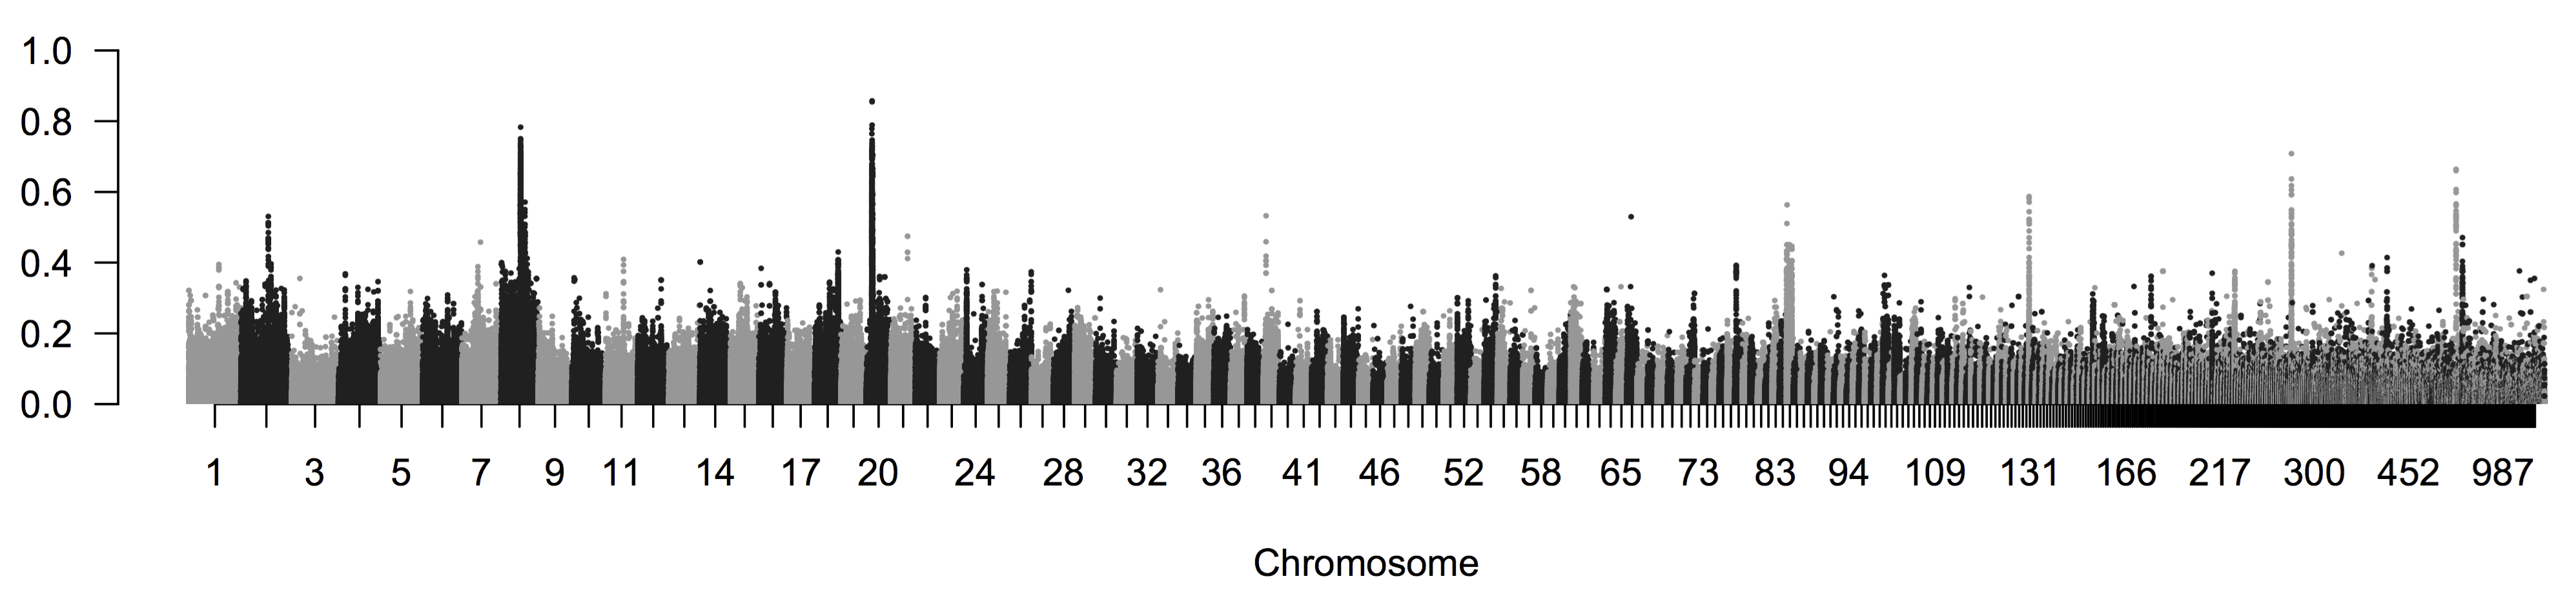
\includegraphics[width = 0.8 \textwidth]{Journal_figs/alleles_genotypes/blue_golden_winged_warblers/GW_FST_warblers.png}  %[width= \marginwidth]
\end{center}
\caption[][-0.5cm]{FST between blue- and golden-winged warbler population samples at SNPs across the genome. Each dot is a SNP, and SNPs are coloured alternating by scaffold. Thanks to David Toews for the figure. } \label{fig:warbler_FST}
\end{figure*}
To illustrate these frequency differences \citet{Toews:16}
genotyped a SNP in each of these high-$F_{ST}$ regions. Here's their
genotyping counts from the SNP, segregating for an allele 1 and 2, in the {\it Wnt}
region, a key regulatory gene involved in feather development:
\begin{center}
  \begin{tabular}{ l c c c}
    & \multicolumn{3}{c}{Genotypes}\\
Species & 11 & 12 & 22\\
\hline
Blue-winged & 2 & 21 & 31\\
Golden-winged & 48 & 12 & 1\\
\hline
\end{tabular}
\end{center}

\begin{question}{}
With reference to the table of {\it Wnt}-allele counts:\\
{\bf A)} Calculate $F_{IS}$ in blue-winged warblers.\\
{\bf B)} Calculate $F_{ST}$ for the sub-population of blue-winged
warblers compared to the combined sample.\\
{ \bf C)} Calculate mean $F_{ST}$ across both sub-populations.
\end{question}

\paragraph{Interpretations of F-statistics}

%JRI: reqriting Fis as covariance is not obvious. could use more explanation. same with Fst as ratio of variances. not immediately obvious how you got there or why those are (co)variances

Let us now return to Wright's definition of the $F$-statistics as correlations
between random gametes, drawn from the same level $X$, relative to level $Y$.
Without loss of generality, we may think about $X$ as individuals and $S$ as
the subpopulation.  Rewriting $\fis$ in terms of the observed homozygote
frequencies ($f_{11}$, $f_{22}$) and expected homozygosities ($p_{S}^2$,
$q_{S}^2$) we find
\begin{equation}
\fis = \frac{2p_Sq_S - f_{12}}{2p_Sq_S} = \frac{f_{11}+f_{22} -
p_S^2 - q_S^2}{2p_Sq_S},
\label{eqn:Fascorr}
\end{equation}
using the fact that $p^2+2pq+q^2=1$, and $f_{12} = 1 - f_{11} - f_{12}$. The
form of eqn.\ (\ref{eqn:Fascorr}) reveals that $\fis$ is the covariance between
pairs of alleles found in an individual, divided by the expected variance under
binomial sampling. Thus, $F$-statistics can be understood as the correlation
between alleles drawn from a population (or an individual) above that expected
by chance (i.e.\ drawing alleles sampled at random from some broader
population). \sidenote[][-2cm]{To see why the numerator of eqn
  \eqref{eqn:Fascorr} is the covariance of a discrete
  random variable see Appendix \eqn \eqref{eqn:binary_covar}, where we
imagine that the random variable is $1$ if the alleles drawn from the
population are the same
and $0$ if not. The denominator is the binomial variance of a sample
of two, and so our equation is a covariance divided by a variance and so
interpretable as a correlation (see \eqn \eqref{eqn:def_corr})}\\

We can also interpret $F$-statistics as proportions of variance explained by
different levels of population structure. To see this, let us think about $\fst$ averaged over $K$
subpopulations, whose frequencies are $p_1,\dots,p_K$. The
frequency in the total population is $p_T=\bar{p} = \nicefrac{1}{K} \sum_{i=1}^K p_i$.
Then, we can
write
\begin{align}
\fst &= \frac{2 \bar{p}\bar{q} - \frac{1}{K}\sum_{i=1}^K 2p_iq_i }{2
\bar{p}\bar{q}} = \frac{ \left(\frac{1}{K} \sum_{i=1}^K p_i^2 +
\frac{1}{K} \sum_{i=1}^K q_i^2 \right) -  \bar{p}^2-\bar{q}^2 }{2
       \bar{p}\bar{q}}  \nonumber\\
       &= \frac{\mathrm{Var}(p_1,\dots,p_K)}{\mathrm{Var}(\bar{p})},
\label{eqn:F_as_propvar}
\end{align}
which shows that $\fst$ is the proportion of the variance explained by the
subpopulation labels. \sidenote[][]{This follows because the
  numerator, in the middle step of \eqn \eqref{eqn:F_as_propvar}, 
is the averaged squared frequency minus the squared frequency, i.e. the
variance (see Appendix \eqn \ref{eqn:sample_var}).}

\subsection{Other approaches to population structure}

There is a broad spectrum of methods to describe patterns of population
structure in population genetic datasets. We'll briefly discuss two
broad-classes of methods that appear often in the literature: assignment methods and principal components analysis.

\subsection{Assignment Methods}

Here we'll describe a simple probabilistic assignment to find the
probability that an individual of unknown population comes from one of
$K$ predefined populations. For example, there are three broad populations
of common chimpanzee ({\it Pan troglodytes}) in Africa: western,
central, and eastern.
%JRI: pic of the subspecies would be fun
Imagine that we have a chimpanzee whose
population of origin is unknown (e.g. it's from an illegal private
collection). If we have genotyped a set of unlinked markers from a panel
of individuals representative of these populations, we can calculate
the probability that our chimp comes from each of these populations. \\

We'll then briefly explain how to extend this idea
to cluster a set of individuals into $K$ initially unknown populations. This
method is a simplified version of what population genetics
clustering algorithms such as STRUCTURE and ADMIXTURE do. \cite{pritchard:00,alexander:09}

\paragraph{A simple assignment method}

We have genotype data from unlinked $S$ biallelic loci for $K$ populations. The
allele frequency of allele $A_1$ at locus $l$ in population $k$ is denoted by
$p_{k,l}$, so that the allele frequencies in population 1 are $p_{1,1},\cdots
p_{1,L}$ and population 2 are $p_{2,1},\cdots p_{2,L}$ and so on.

You genotype a new individual from an unknown population at these $L$ loci. This individual's genotype at locus $l$ is $g_l$, where $g_l$ denotes the number of copies of allele $A_1$ this individual carries at this locus ($g_l=0,1,2$).
%JRI: is this formally the definition of a set? should if be $g_l={0,1,2}$ ?

The probability of this individual's genotype at locus $l$ conditional on coming from population $k$, i.e. their alleles being a random HW draw from population $k$, is
\begin{equation}
  P(g_l | \textrm{pop k}) =
  \begin{cases}
(1-p_{k,l})^2  & g_l=0 \\
2 p_{k,l} (1-p_{k,l}) & g_l=1\\
p_{k,l}^2  & g_l=2
\end{cases}
\end{equation}

Assuming that the loci are independent, the probability of the individual's genotype across all S loci, conditional on the individual coming from population $k$, is
\begin{equation}
P(\textrm{ind.} | \textrm{pop k})  = \prod_{l=1}^S P(g_l | \textrm{pop k}) \label{eqn_assignment}
\end{equation}

% TODO: deleted "new" in bayes -- this is confusing I think for students
We wish to know the probability that this new individual comes from population
$k$, i.e. $P(\textrm{pop k} | \textrm{ind.})$. We can obtain this through Bayes'
rule

\begin{equation}
 P(\textrm{pop k} | \textrm{ind.})  = \frac{P(\textrm{ind.} | \textrm{pop k}) P(\textrm{pop k})}{P(\textrm{ind.})}
\end{equation}
where
\begin{equation}
P(\textrm{ind.}) = \sum_{k=1}^K  P(\textrm{ind.} | \textrm{pop k}) P(\textrm{pop k})
\end{equation}
is the normalizing constant.\sidenote{See the Appendix
  \eqref{eqn:Bayes_Rule} for more on Bayes' Rule} We can interpret $P(\textrm{pop k})$ as the
prior probability of the individual coming from population $k$, and unless
we have some other prior knowledge we will assume that the new individual has a equal probability of coming from each population $P(\textrm{pop k})=\nicefrac{1}{K}$.

We interpret
\begin{equation}
 P(\textrm{pop k} | \textrm{ind.})
\end{equation}
as the posterior probability that our new individual comes from each of our $1,\cdots, K$ populations.

More sophisticated versions of this are now used to allow for hybrids,
e.g, we can have a proportion $q_k$ of our individual's genome come
from population $k$ and estimate the set of $q_k$'s.

%{\bf Q}\arabic{Question} \refstepcounter{Question}
\begin{question}{}

Returning to our chimp example, imagine that we have genotyped a set of
individuals from the Western and Eastern populations at two SNPs (we'll ignore
the central population to keep things simpler).
%JRI: in previous examples you use A1A2 not Aa. I would pick one convention and stick with it.
The frequency of the capital allele at two SNPs ($A/a$ and $B/b$) is given by

\begin{center}
\begin{tabular}{|ccc|}
\hline
Population & locus A & locus B \\
\hline
Western & $0.1$ & $0.85$ \\
Eastern  & $0.95$ & $0.2$ \\
%Eastern & $0.5$ & $0.5$ \\
\hline
\end{tabular}
\end{center}
%JRI: no answer to this question in answer key
%



 %Archives du Mus{\'e}um d'Histoire Naturelle, Paris. Tom 101858
%https://www.flickr.com/photos/biodivlibrary/19930229848/in/photolist-XGMmmV-wnaCYy-wDMHFP-dpNAc7-bw9qDC-bw9orQ-bJPuCF-eV4etD-d9s1By-cbcysm-c5izpA-bvSkgm-bu7ij8-azL7vS-ayF5zC-atDTpg-atDTuz-akH6mL-ag15Rf-ag15Lb
 
{\bf A)} Our individual, whose origin is unknown, has the genotype $AA$ at the
first locus and $bb$ at the second. What is the posterior probability that our
individual comes from the Western population versus Eastern chimp population?\\[1 em]
%
{\bf B)} (Trickier) Lets assume that our individual from part A is a
hybrid (not necessarily an F1). At each locus, with probability $q_W$ our individual draws an allele
from the Western population and with probability $q_E=1-q_W$ they draw an
allele from the Eastern population. What is the probability of our individual's
genotype given $q_W$? \\

{\bf Optional} You could plot this probability as a function of $q_W$. How does
your plot change if our individual is heterozygous at both loci?
\end{question}

\begin{marginfigure}
\begin{center}
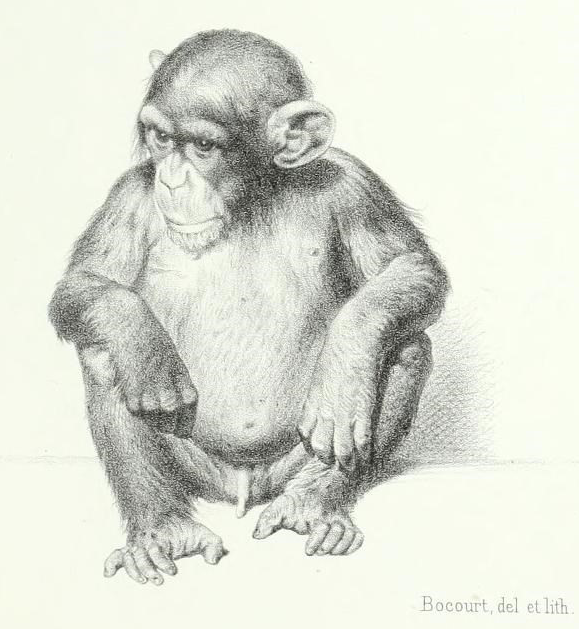
\includegraphics[width=\textwidth]{Journal_figs/alleles_genotypes/chimp/chimp.png}
\end{center}
\caption{Chimpanzee. }
  \label{chimp_pic}
\end{marginfigure}


\paragraph{Clustering based on assignment methods}
\graham{Possible to make figure showing structure converging?}
While it is great to be able to assign our individuals to a particular
population, these ideas can be pushed to learn about how best to describe our
genotype data in terms of discrete populations without assigning any of our
individuals to populations {\it a priori}.  We wish to cluster our individuals
into $K$ unknown populations. We begin by assigning our individuals at random
to these $K$ populations.
\begin{enumerate}
\item Given these assignments we estimate the allele frequencies at all of our loci in each population.
\item Given these allele frequencies we chose to reassign each individual to a population $k$ with a probability given by \eqn \eqref{eqn_assignment}.
\end{enumerate}
We iterate steps 1 and 2 for many iterations (technically, this approach is known as \emph{Gibbs Sampling}). If the data is
sufficiently informative, the assignments and allele frequencies will
quickly converge on a set of likely population assignments and allele
frequencies for these populations.
\begin{figure}
% TODO: MISSING FIGURE
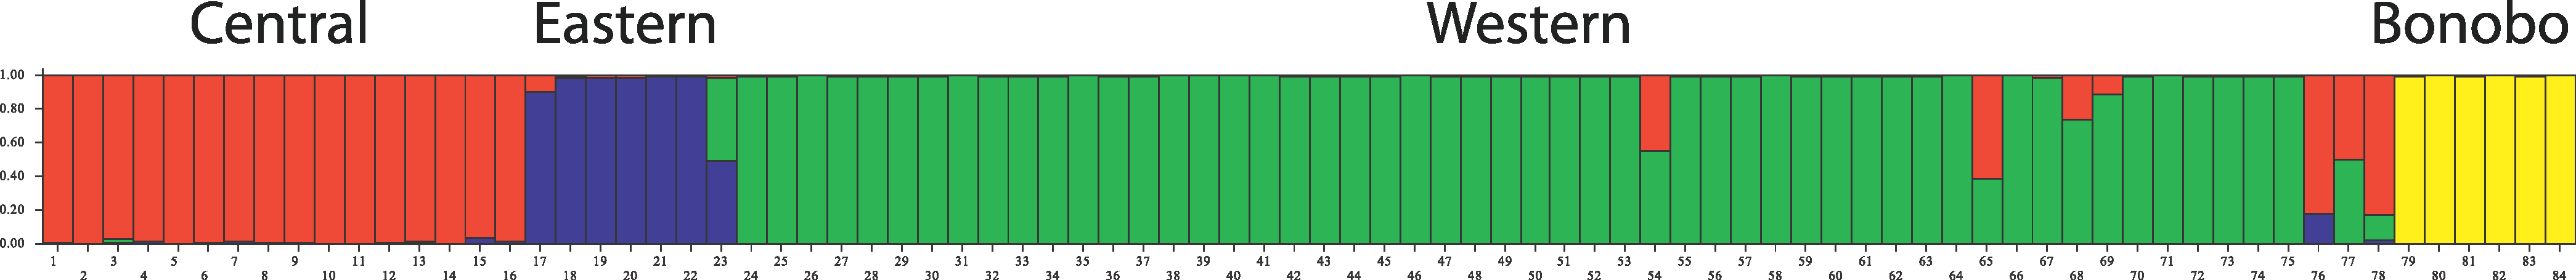
\includegraphics[width= \textwidth, height = 0.12 \textheight]{figures/Becquet_et_al_STRUCTURE_journal_pgen_0030066_g001.png}
\caption{ \citet{becquet:07} genotyped 78 common chimpanzee and 6 bonobo at
over 300 polymorphic markers (in this case microsatellites). They ran STRUCTURE to cluster the individuals
using these data into $K=4$
populations. In \citet{becquet:07} above figure they show each individual as a
vertical bar divided into four colours depicting the estimate of the fraction
of ancestry that each individual draws from each of the four
estimated populations  (\PLOSccBY). We can see that these four colours/populations correspond to: Red, central; blue, eastern; green,
western; yellow, bonobo. } \label{fig:chimp_structure}
%In their caption of this figure they say:
%{\it ``STRUCTURE Analysis, Blinded to Population Labels, Recapitulates the Reported Population Structure of the Chimpanzees
%Individuals 76–-78 are reported hybrids. Only two individuals with a
%$>5\%$ proportion of ancestry in more than one inferred cluster are wild
%born: number 54 and number 17.''}}  % http://journals.plos.org/plosgenetics/article?id=10.1371%2Fjournal.pgen.0030066
%=======
%Individuals 76–78 are reported hybrids. Only two individuals with a $>5\%$ proportion of ancestry in more than one inferred cluster are wild born: number 54 and number 17. Red, central; blue, eastern; green, western; yellow, bonobo.''}
\end{figure}

To do this in a full Bayesian scheme we need to place priors on the allele
frequencies (for example, one could use a beta distribution prior). Technically
we are using the joint posterior of our allele frequencies and
assignments. Programs like STRUCTURE, use this type of algorithm to
cluster the individuals in an ``unsupervised'' manner (i.e. they work
out how to assign individuals to an unknown set of populations).  See Figure \ref{fig:chimp_structure} for an example of
\citeauthor{becquet:07} using STRUCTURE to determine the population structure of chimpanzees.

STRUCTURE-like methods have proven incredible popular and useful in examining population structure within species. However, the results of these methods are open to misinterpretation; see \citet{lawson:18} for a recent discussion. Two common mistakes are 1) taking the results of STRUCTURE-like approaches for some particular value of K and taking this to represent the best way to describe population-genetic variation. 2) Thinking that these clusters represent `pure' ancestral populations.

There is no right choice of K, the number of clusters to partition into. There are methods of judging the `best' K by some statistical measure given some particular dataset, but that is not the same as saying this is the most meaningful level on which to summarize population structure in data. For example, running STRUCTURE on world-wide human populations for low value of K will result in population clusters that roughly align with continental populations \citep{rosenberg:02}. However, that does not tell us that assigning ancestry at the level of continents is a particularly meaningful way of partitioning individuals. Running the same data for higher value of K, or within continental regions, will result in much finer-scale partitioning of continental groups \citep{rosenberg:02,li:08}. No one of these layers of population structure identified is privileged as being more meaningful than another.

It is tempting to think of these clusters as representing ancestral populations, which themselves are  not the result of admixture. However, that is not the case, for example, running STRUCTURE on world-wide human data identifies a cluster that contains many European individuals, however, on the basis of ancient DNA we know that modern Europeans are a mixture of distinct ancestral groups.

\subsection{Principal components analysis}
Principal component analysis (PCA) is a common statistical approach to visualize  high dimensional data, and used by many fields. The idea of PCA is to give a location to each individual data-point on each of a small number principal component axes. These PC axes are chosen to reflect major axes of variation in the data,
  with the first PC being that which explains largest variance, the second the second most, and so on. The use of PCA in population genetics was
pioneered by Cavalli-Sforza and colleagues and now with large genotyping datasets, PCA has made a comeback. \cite{menozzi:78,patterson:06}
% TODO: citations.

Consider a dataset consisting of N individuals at $S$ biallelic SNPs. The
$i^{th}$ individual's genotype data at locus $\ell$ takes a value
$g_{i,\ell}=0,1,\; \text{or} \; 2$ (corresponding to the number of copies of
allele $A_1$ an individual carries at this SNP). We can think of this as a $N
\times S$ matrix (where usually $N \ll S$).
%JRI: here you assume reader knows SNP/locus can be used interchangeably

Denoting the sample mean allele frequency at SNP $\ell$ by $p_{\ell}$, it's
common to standardize the genotype in the following way
\begin{equation}
  \frac{g_{i,\ell} - 2 p_{\ell}}{\sqrt{2 p_{\ell}(1-p_{\ell})}} \label{eqn:std_allele_freq}
\end{equation}
i.e.
at each SNP we center the genotypes by subtracting the mean genotype
($2p_{\ell}$) and divide through by the square root of the expected variance assuming that
alleles are sampled binomially from the mean frequency ($\sqrt{2 p_{\ell}
  (1-p_{\ell})}$). Doing this to all of our genotypes, we form a data matrix (of
  dimension $N \times S$). We can then perform principal component analysis of
  this data matrix to uncover the major axes of genotype variance in our
  sample. Figure \ref{fig:chimp_PCA} shows a PCA from \citet{becquet:07} using the same chimpanzee data as in Figure \ref{fig:chimp_structure}.

\begin{figure}
% TODO: MISSING FIGURE
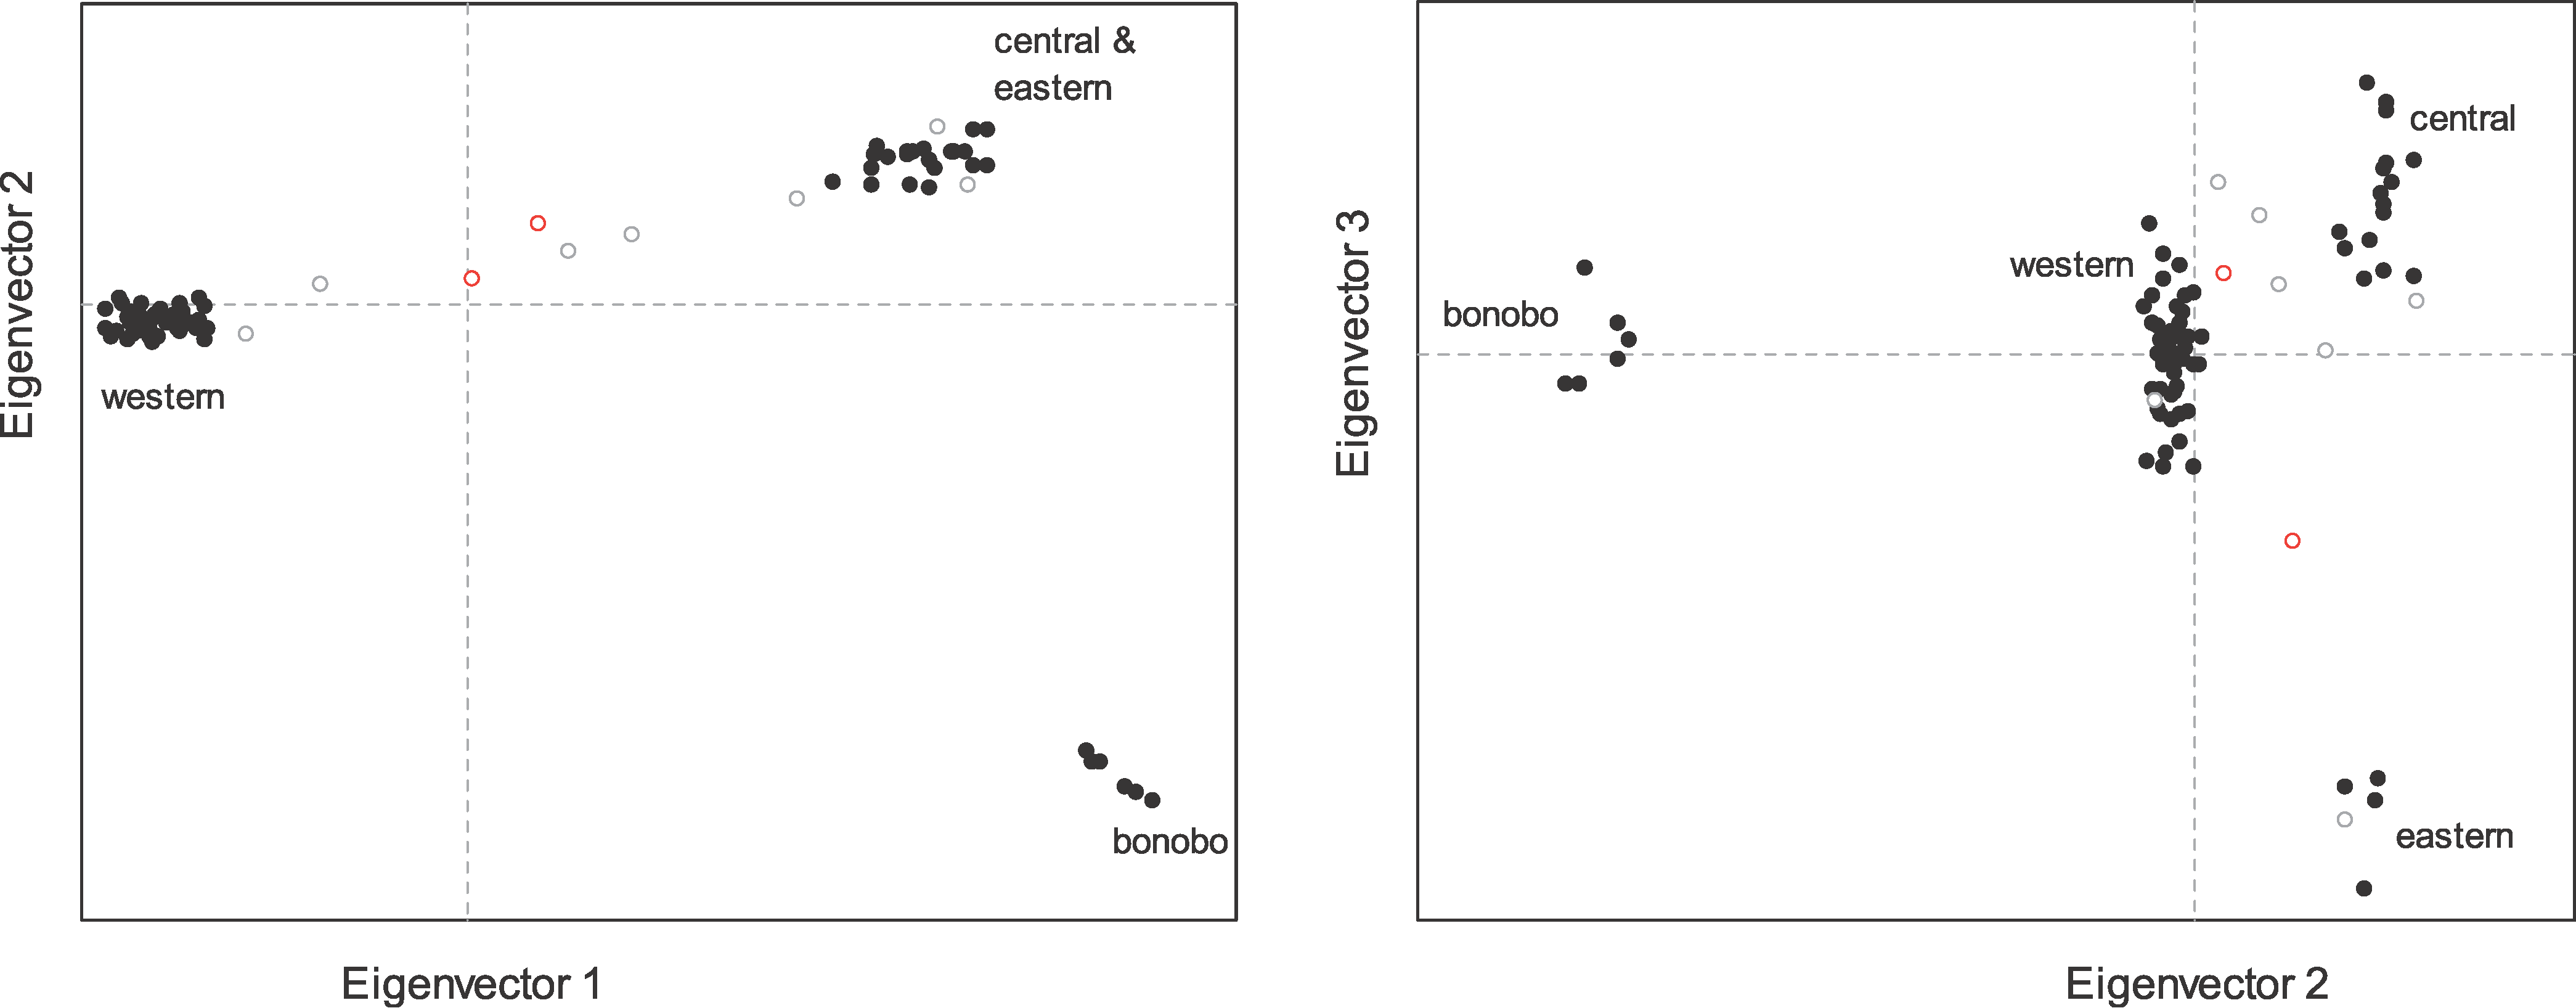
\includegraphics[width=
  \textwidth]{figures/Becquet_et_al_STRUCTURE_journal_pgen_0030066_g002.png}
  \caption{ Principal Component Analysis by  \citet{becquet:07} using the same chimpanzee data as in Figure
    \ref{fig:chimp_structure}. Here  \citet{becquet:07}  plot the location of each individual
    on the first two principal components (called eigenvectors) in the left
    panel, and on the second and third principal components (eigenvectors) in
    the right panel (\PLOSccBY). In the PCA,  individuals identified as all of one ancestry by STRUCTURE cluster together by population (solid circles). While the nine individuals identified by STRUCTURE as hybrids (open circles) for the
      most part fall at intermediate locations in the PCA. There are two individuals
      (red open circles) reported as being of a particular population but that
      but appear to be hybrids.} \label{fig:chimp_PCA}
\end{figure}


  It is worth taking a moment to delve further into what we are doing
here. There's a number of equivalent ways of thinking about what PCA
is doing. One of these ways is to think that when we do PCA we are building the individual by individual
covariance matrix and performing an eigenvalue decomposition of this
matrix (with the eigenvectors being the PCs).  This individual by individual covariance matrix has entries
the $[i,~j]$ given by
\begin{equation}
\frac{1 }{S-1} \sum_{\ell=1}^S \frac{(g_{i,\ell} - 2p_{\ell})(g_{j,\ell} -
  2p_{\ell})}{2 p_{\ell}(1-p_{\ell})} \label{eqn:kinship_mat}
\end{equation}
Note that this is the sample covariance of our standardized allele
frequencies (\eqn \eqref{eqn:std_allele_freq}), and is very similar to those we
encountered in discussing $F$-statistics as correlations (\eqn
\eqref{eqn:Fascorr}), except now we are asking about the covariance
between two individuals above that expected if they were both drawn
from the total sample at random (rather than the covariance of alleles
within a single individual). So by performing PCA on the data we are
learning about the major (orthogonal) axes of the kinship matrix.


As an example of the application of PCA, let's consider the case of the
putative ring species in the greenish warbler ({\it Phylloscopus
  trochiloides}) species complex. This set of subspecies exists in a
ring around the edge of the Himalayan plateau. \citet{alcaide:14}
collected $95$ greenish warbler samples from $22$ sites around the
ring, and the sampling locations are shown in Figure \ref{fig:Gwarbler_geo}.
\begin{figure}
\begin{center}
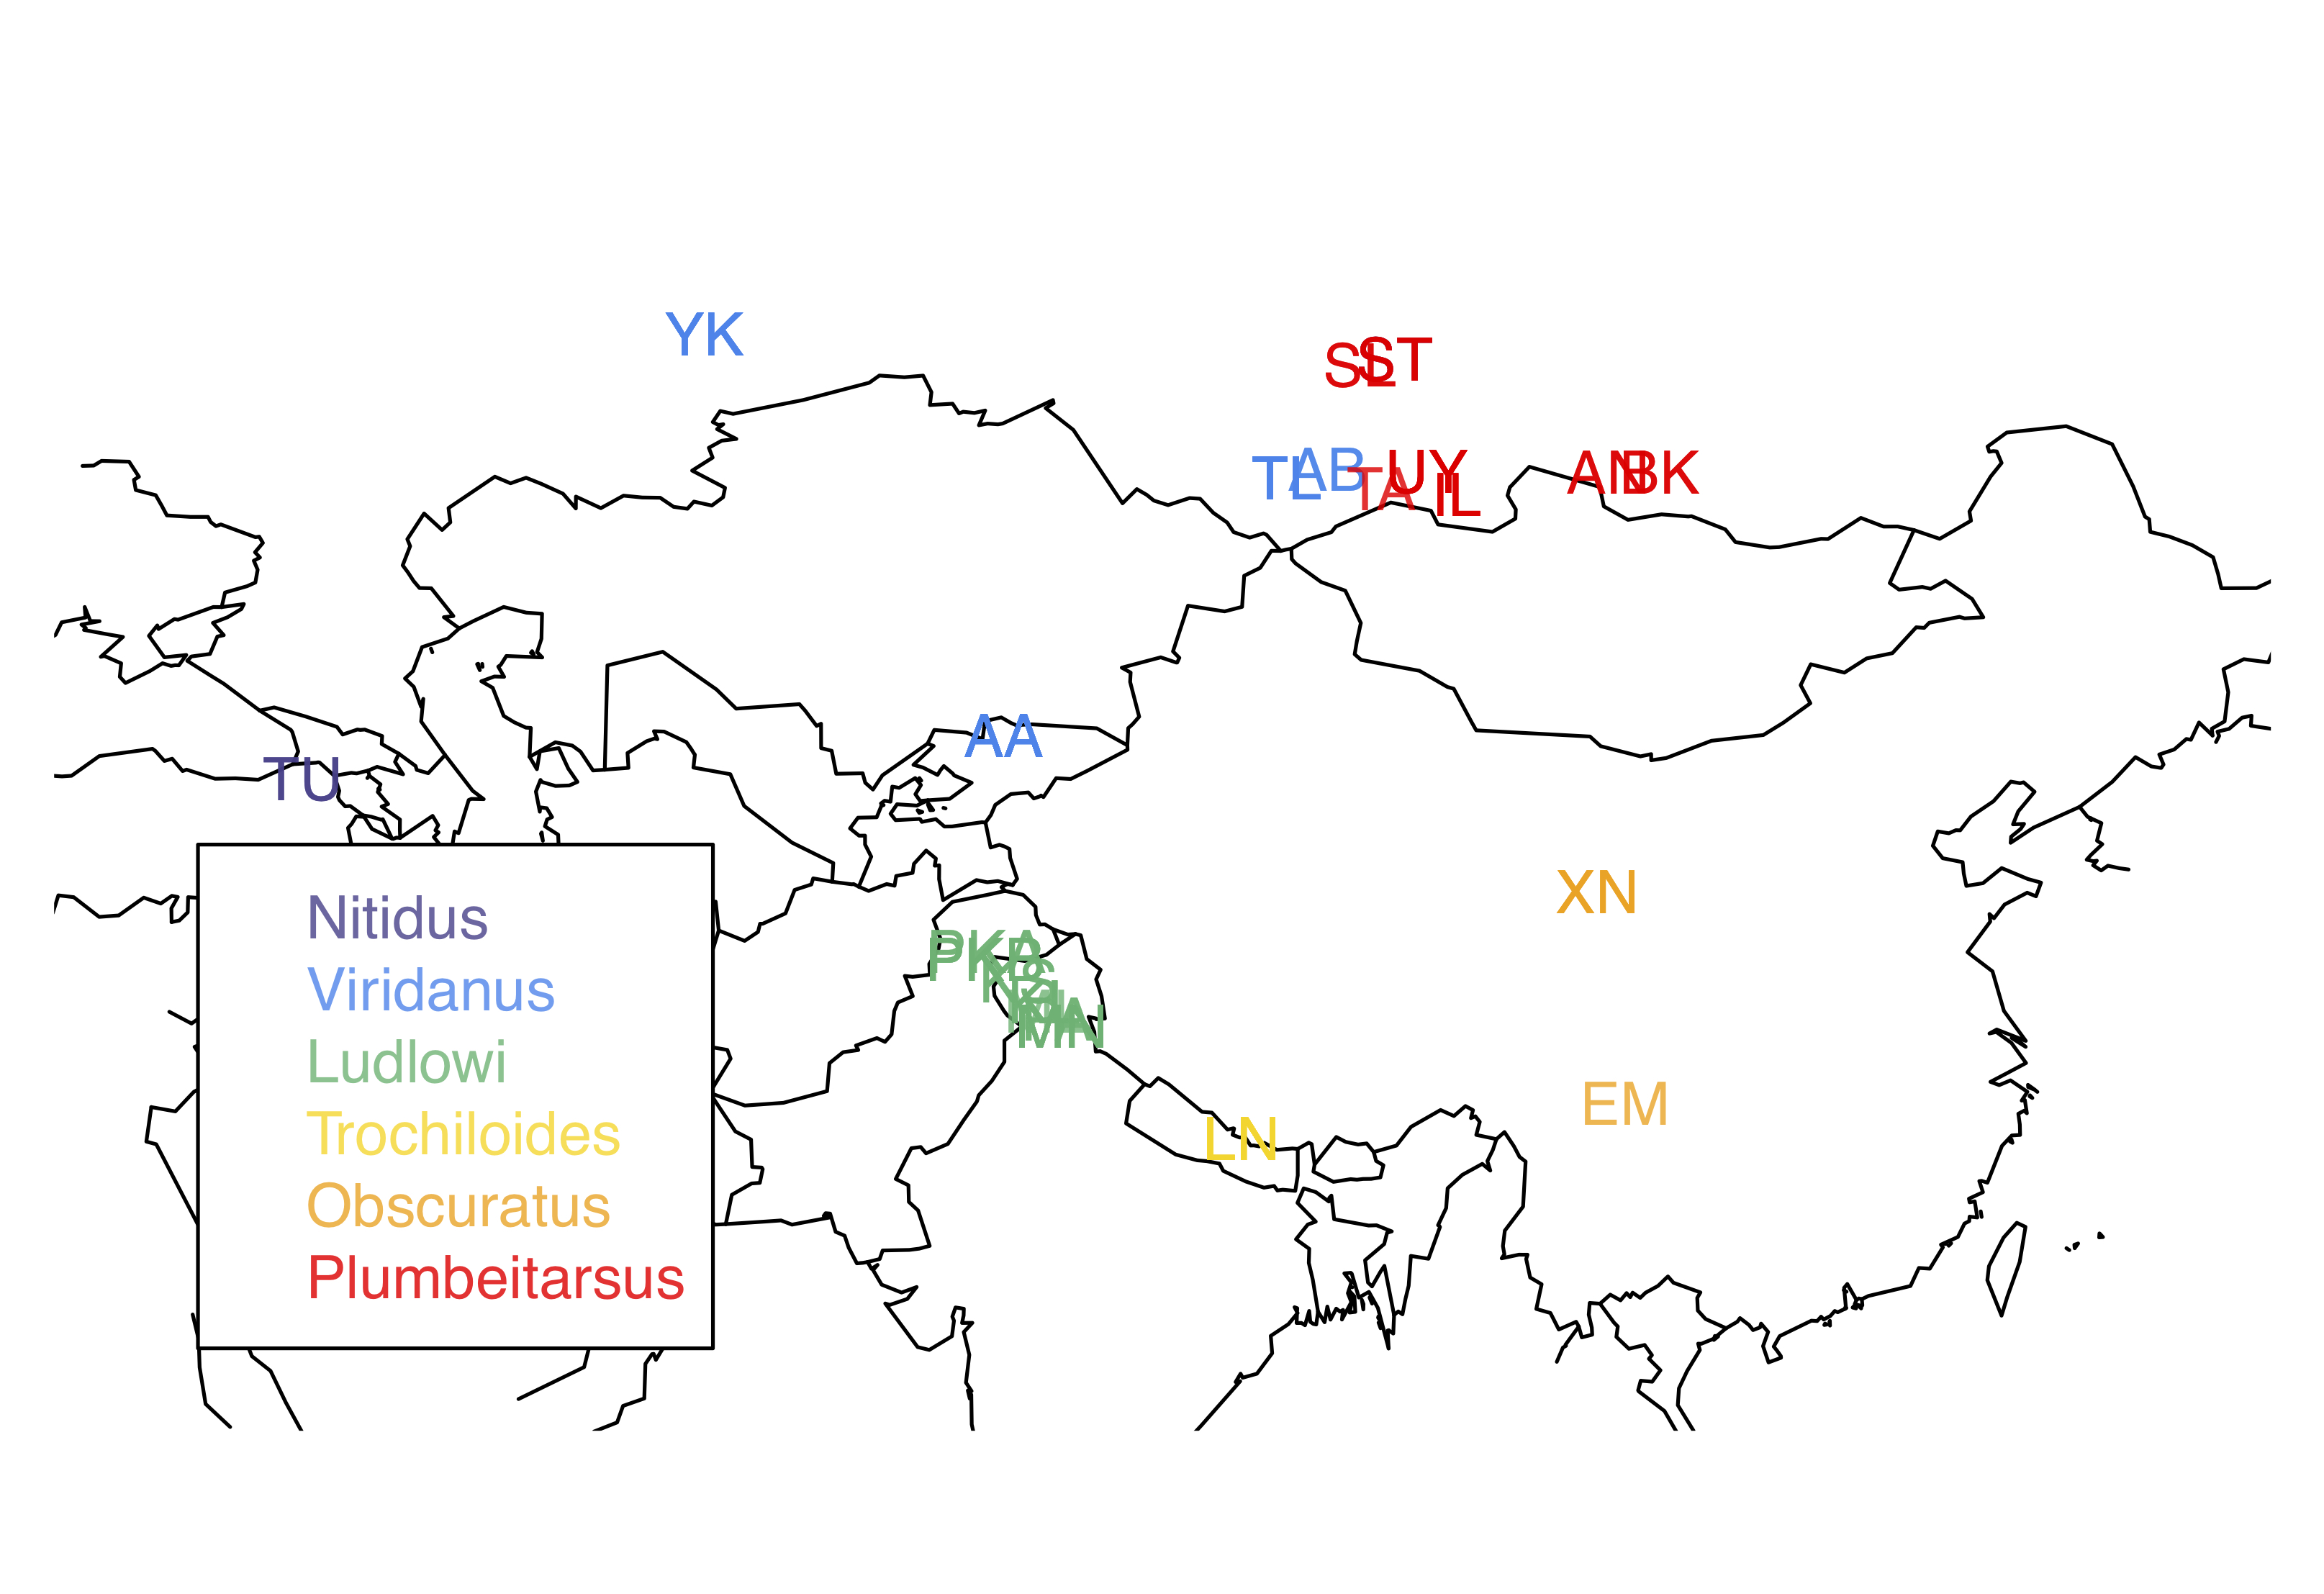
\includegraphics[width= 0.75 \textwidth]{figures/warbler_PCA_figs/warbler_geo_map.jpg}
\end{center}
    \caption[][-0cm]{The sampling locations of 22 populations of greenish warblers from \citet{alcaide:14}. The samples are coloured by the subspecies. \gitcode{https://github.com/cooplab/popgen-notes/blob/master/Rcode/warblerdata/warbler_ind_PCA.R}}
\label{fig:Gwarbler_geo}
\end{figure}


It is
thought that these warblers spread from the south, northward in two different directions around the inhospitable Himalayan
plateau, establishing populations along the western edge
(green and blue populations) and the eastern edge (yellow and red
populations). When they came into secondary contact
in Siberia, they were reproductively isolated from one another, having
evolved different songs and accumulated other reproductive barriers
from each other as they spread independently north around the
plateau, such that {\it P. t. viridanus} (blue) and {\it P. t. plumbeitarsus}
(red) populations presently form a stable hybrid zone.


\citet{alcaide:14} obtained sequence data for their samples at 2,334 snps. In Figure \ref{fig:warbler_heat}
you can see the matrix of kinship coefficients, using \eqn \eqref{eqn:kinship_mat}, between all pairs of
samples. You can already see a lot about population structure in this
matrix. Note how the red and yellow samples, thought to be derived from
the Eastern route around the Himalayas, have higher kinship with each
other, and blue and the (majority) of the green samples, from the Western route, form a
similarly close group in terms of their higher kinship.
\begin{marginfigure}[-5cm]
% TODO: MISSING FIGURE
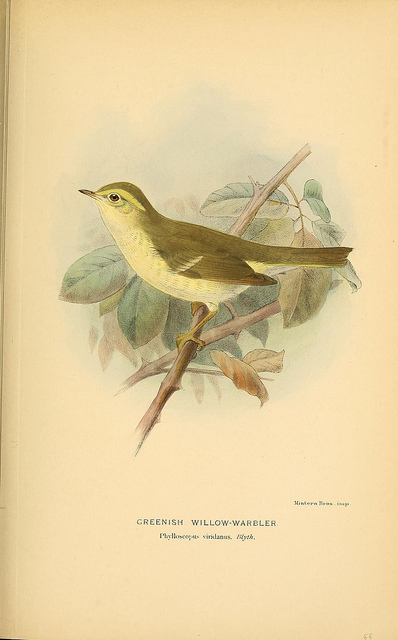
\includegraphics[width= \textwidth]{illustration_images/alleles_genotypes/greenish_warbler/10036311396_14915d1715_z.jpg}
  \caption{Greenish warbler, subspp. viridanus ({\it Phylloscopus
      trochiloides viridanus}). \BHLNC{Coloured figures of the birds of the
    British Islands. 1885. Lilford T. L. P..}{https://www.biodiversitylibrary.org/page/34576931\#page/147/mode/1up}{American Museum of Natural History Library} (Greenish warblers are
    rare visitors to the UK.)}\label{fig:greenish_warbler}   %https://www.flickr.com/photos/biodivlibrary/10036311396/in/photolist-ghSHHE
\end{marginfigure}

\begin{figure}
\begin{center}
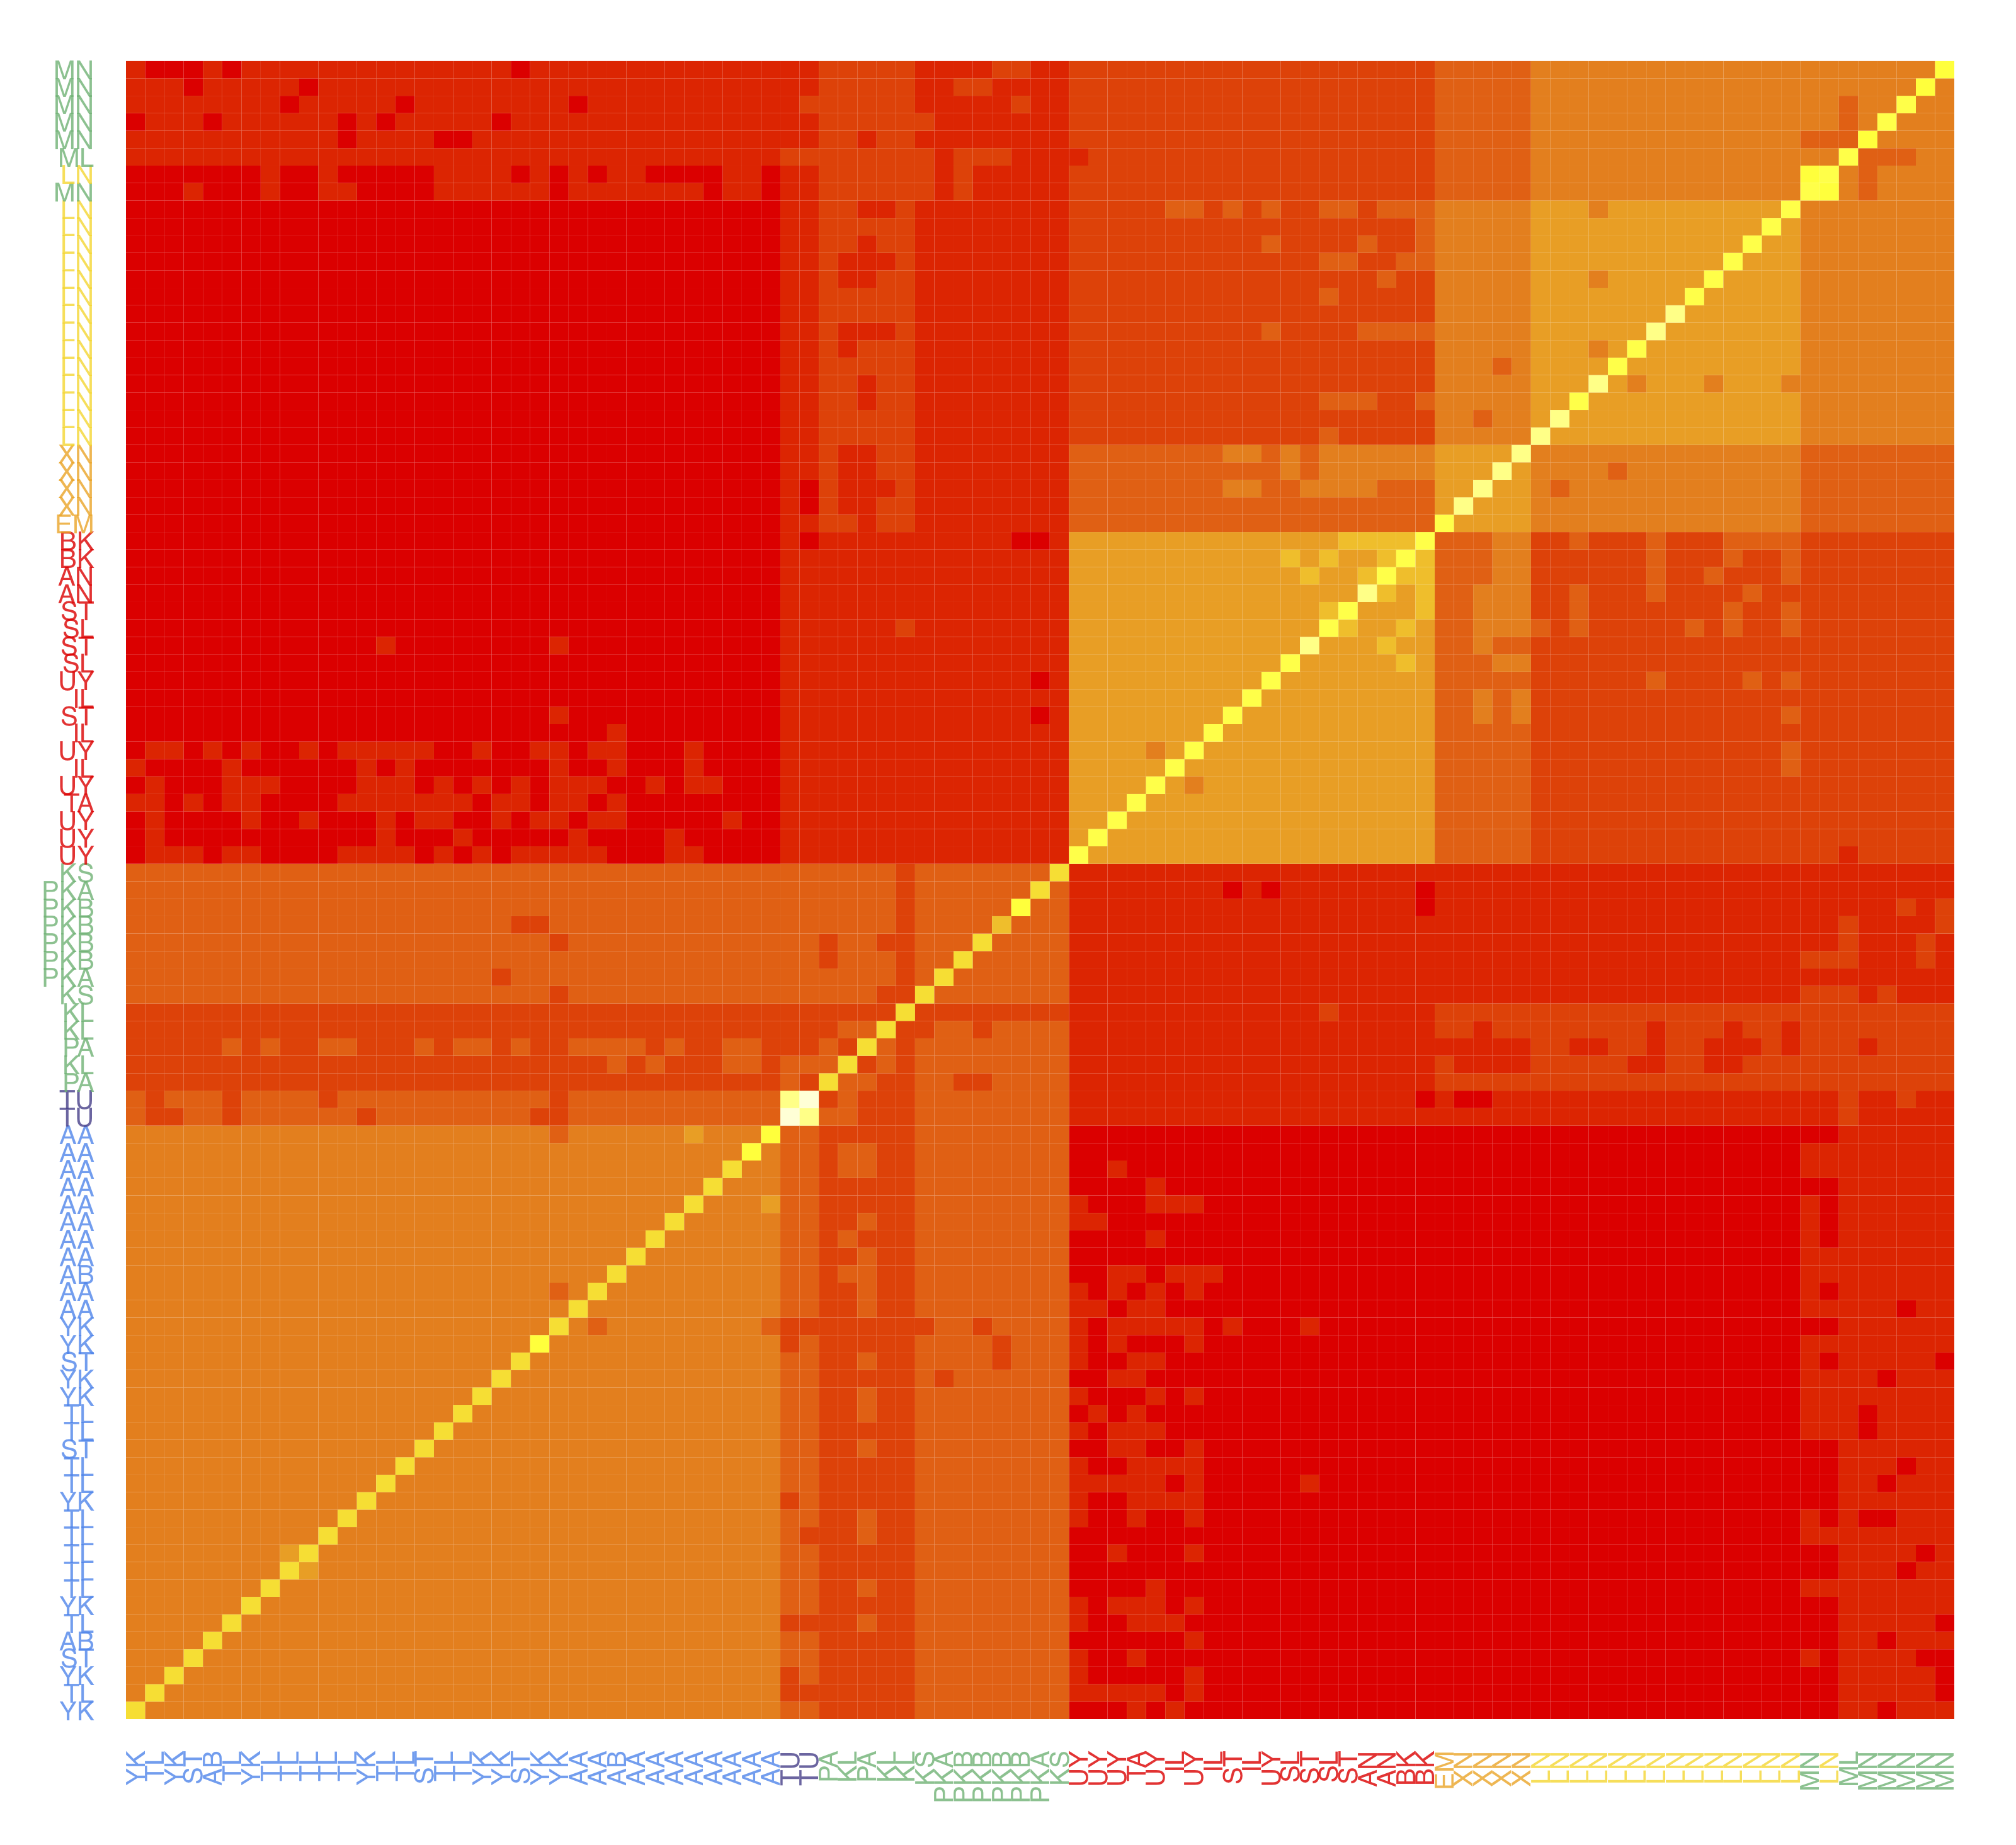
\includegraphics[width=
  0.75 \textwidth]{figures/warbler_PCA_figs/warbler_heatmap.png}
  \end{center}
    \caption[][3cm]{The matrix of kinship coefficients calcuated for the 95
      samples of greenish warblers. Each cell in the matrix gives the
      pairwise kinship coefficient calculated for a particular pair. Hotter colours indicating higher
      kinship. The $x$ and $y$ labels of individuals are the population labels from Figure \ref{fig:Gwarbler_geo}, and coloured by subspecies label as in that figure. The rows and columns have been
    organized to cluster individuals with high kinship.  \gitcode{https://github.com/cooplab/popgen-notes/blob/master/Rcode/warblerdata/warbler_ind_PCA.R}}
\label{fig:warbler_heat}
\end{figure}

We can then perform PCA on this kinship matrix to identify the major
axes of variation in the dataset. Figure \ref{fig:warbler_PCA} shows
the samples plotted on the first two PCs.
\begin{figure}
\begin{center}
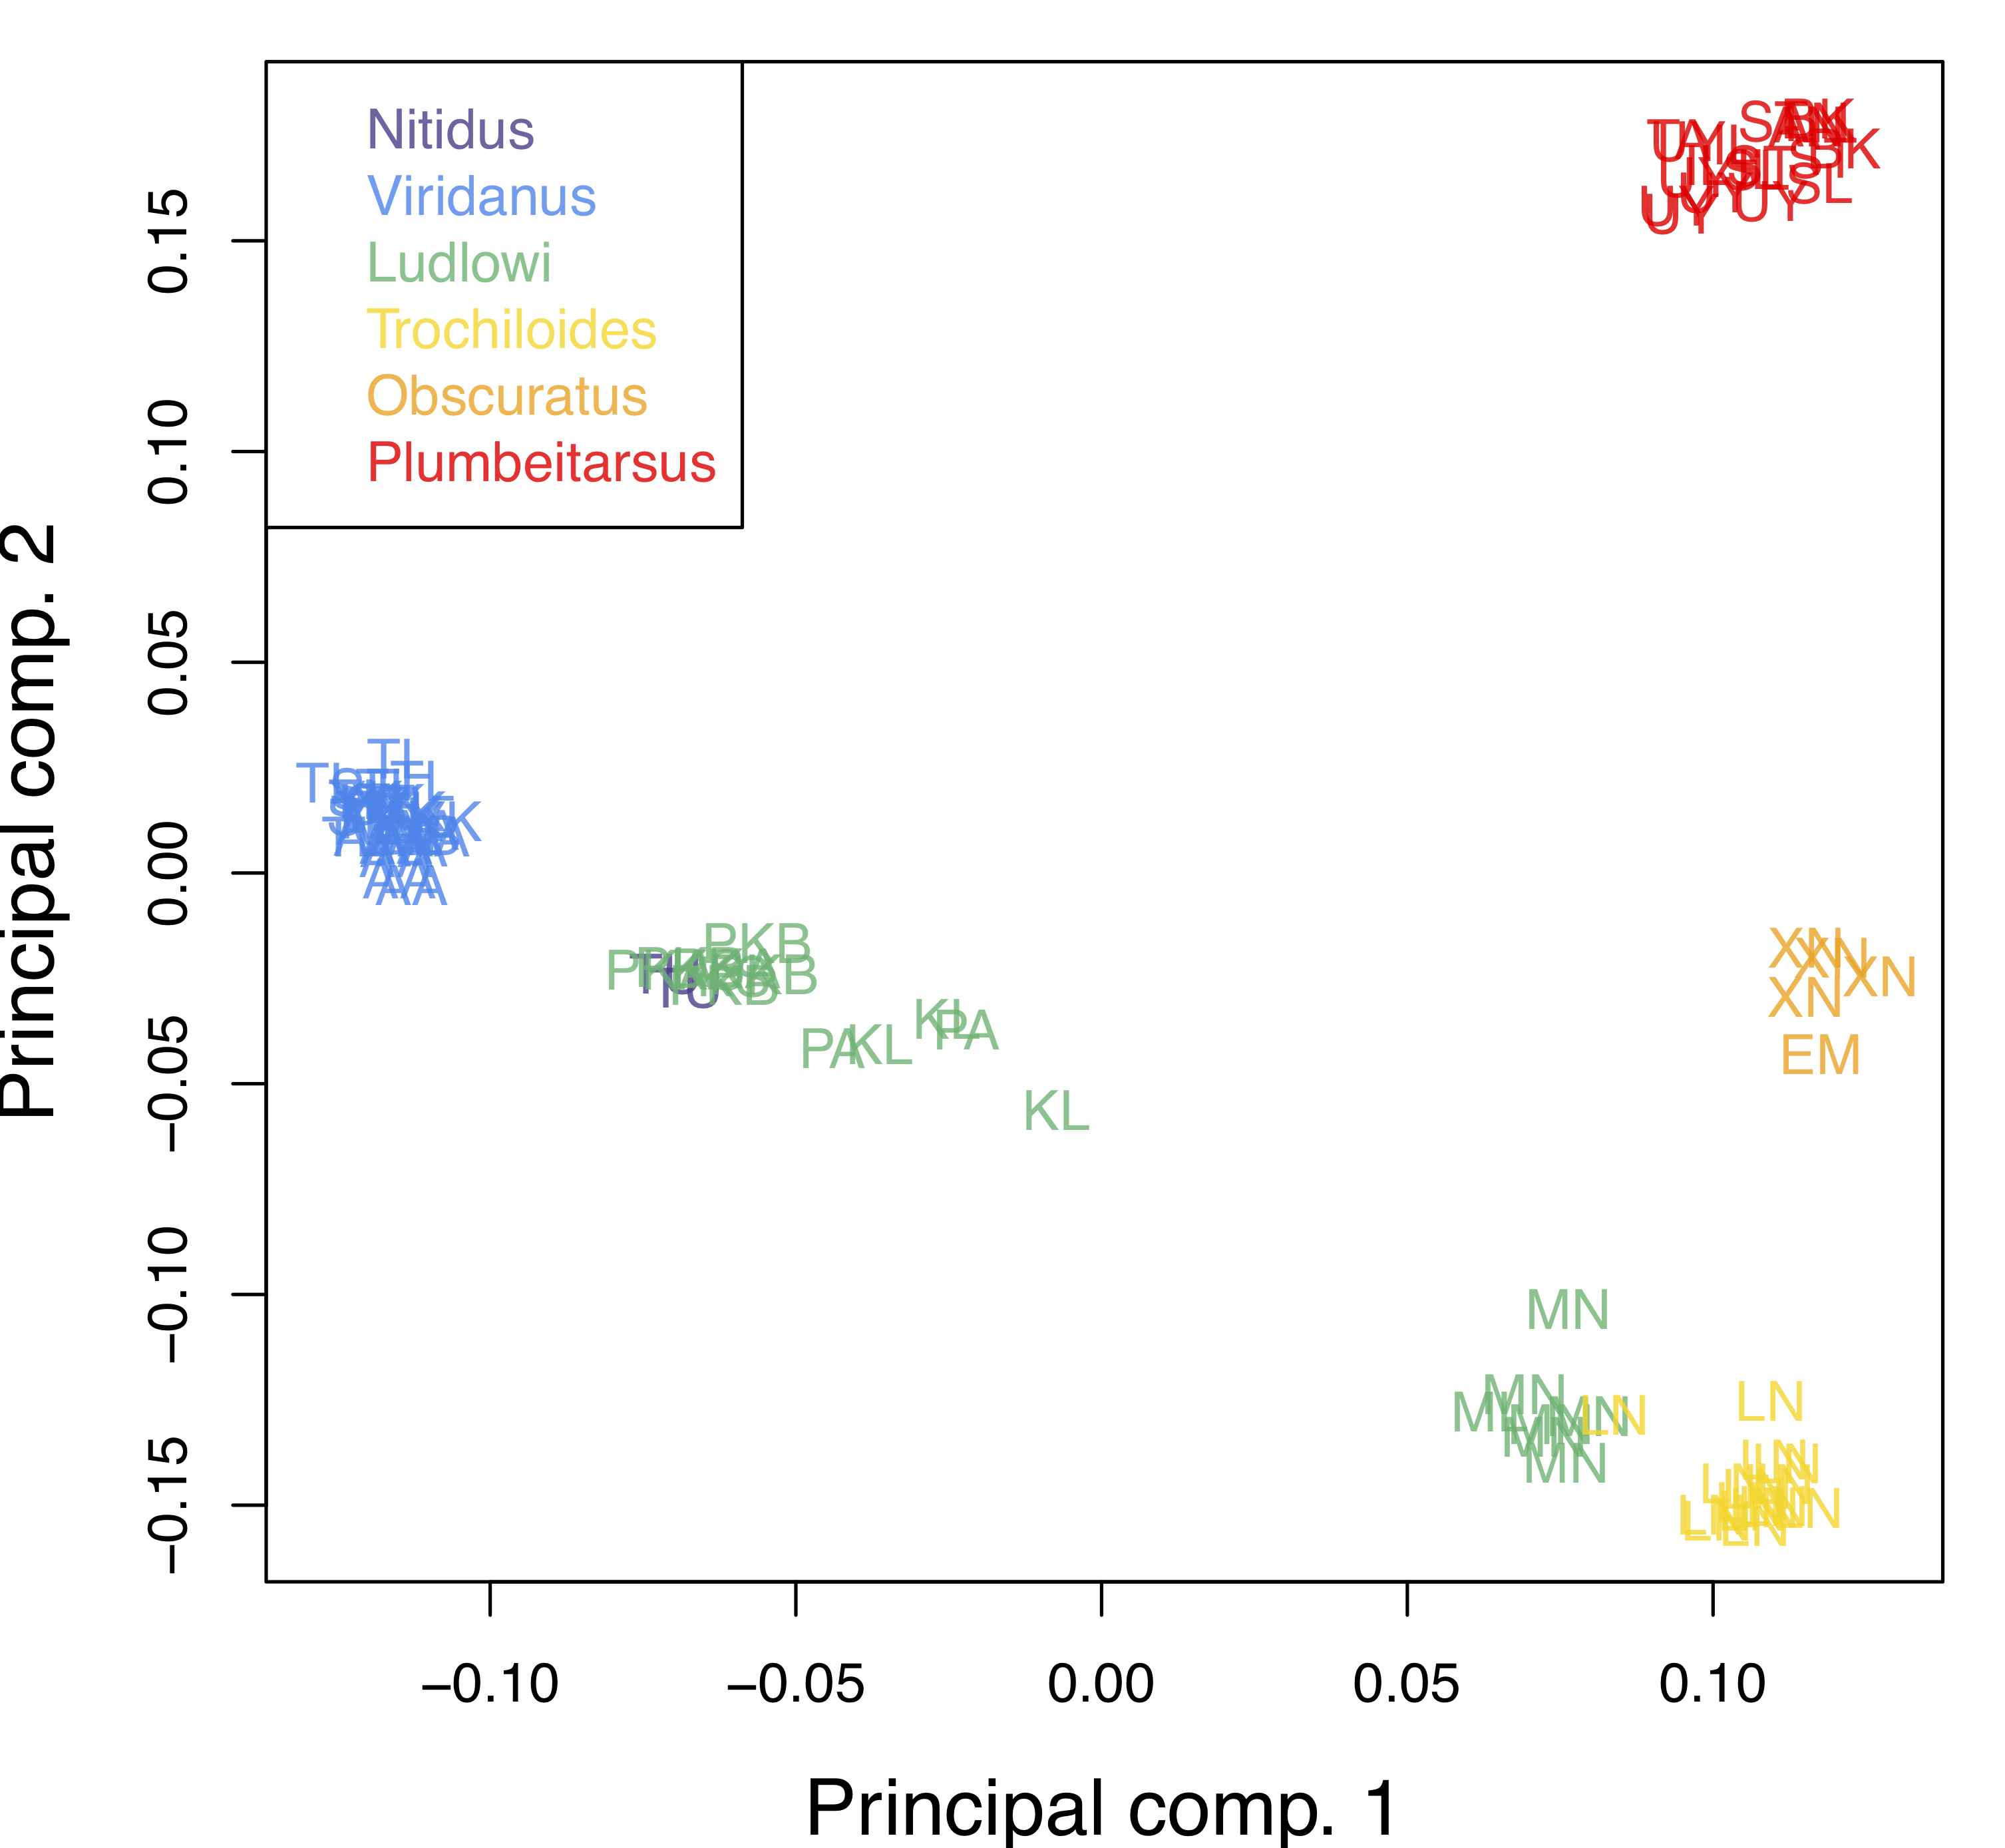
\includegraphics[width=
  0.75 \textwidth]{figures/warbler_PCA_figs/warbler_PCAmap.jpg}
  \end{center}
    \caption{ The 95 greenish warbler samples plotted on their
      locations on the first two principal components. The labels of
      individuals are the population labels from Figure
      \ref{fig:Gwarbler_geo}, and coloured by subspecies label as in
      that figure. \gitcode{https://github.com/cooplab/popgen-notes/blob/master/Rcode/warblerdata/warbler_ind_PCA.R}}
\label{fig:warbler_PCA}
\end{figure}
The two major routes of expansion clearly occupy different parts of PC space. The first principal component distinguishes populations running North to South along the western route of expansion, while the second principal component distinguishes among populations running North to South along the  Eastern route of expansion. Thus genetic data supports the hypothesis that the greenish warblers speciated as they moved around the Himalayan
plateau. However, as noted by \citet{alcaide:14}, it also suggests additional complications to the traditional view of these warblers as an unbroken ring species, a case of speciation by continuous geographic isolation. The {\it Ludlowi} subspecies shows a significant genetic break, with the southern most MN samples clustering with the {\it Trochiloides} subspecies, in both the PCA and kinship matrix (Figures \ref{fig:warbler_PCA} and \ref{fig:warbler_heat}), despite being much more geographically close to the other {\it Ludlowi} samples. This suggests that genetic isolation is not just a result of geographic distance, and other biogeographic barriers must be considered in the case of this broken ring species.

Finally, while PCA is a wonderful tool for visualizing genetic data, care must be taken in its interpretation. The U-like shape in the case of the greenish warbler PC might be consistent with some low level of gene flow between the red and the blue populations, pulling them genetically closer together and helping to form a genetic ring as well as a geographic ring. However, U-like shapes are expected to appear in PCAs even if our populations are just arrayed along a line, and more complex geometric arrangements of populations in PC space can result under simple geographic models \citep{novembre:08}. Inferring the geographical and population-genetic history of species requires the application of a range of tools; see \citet{alcaide:14} and \citet{bradburd:16} for more discussion of the greenish warblers.


%For example, it would be tempting to see the U shape in the warbler example (Figure \ref{fig:warbler_PCA}) as representing a
% \label{fig:chimp_PCA}

% % http://journals.plos.org/plosgenetics/article?id=10.1371%2Fjournal.pgen.0030066
% %======= Individuals 76–78 are reported hybrids. Only two individuals with a
% %$>5\%$ proportion of ancestry in more than one inferred cluster are wild born:
% %number 54 and number 17. Red, central; blue, eastern; green, western; yellow,
% %bonobo.''}
% \end{figure}

\newpage
\subsection{Correlations between loci, linkage disequilibrium, and recombination}

%</source-file>

Up to now we have been interested in correlations between alleles at the same
locus, e.g. correlations within individuals (inbreeding) or between individuals
(relatedness). We have seen how relatedness between parents affects the extent
to which their offspring is inbred. We now turn to correlations between alleles
at different loci.\\

\begin{marginfigure}
\begin{center}
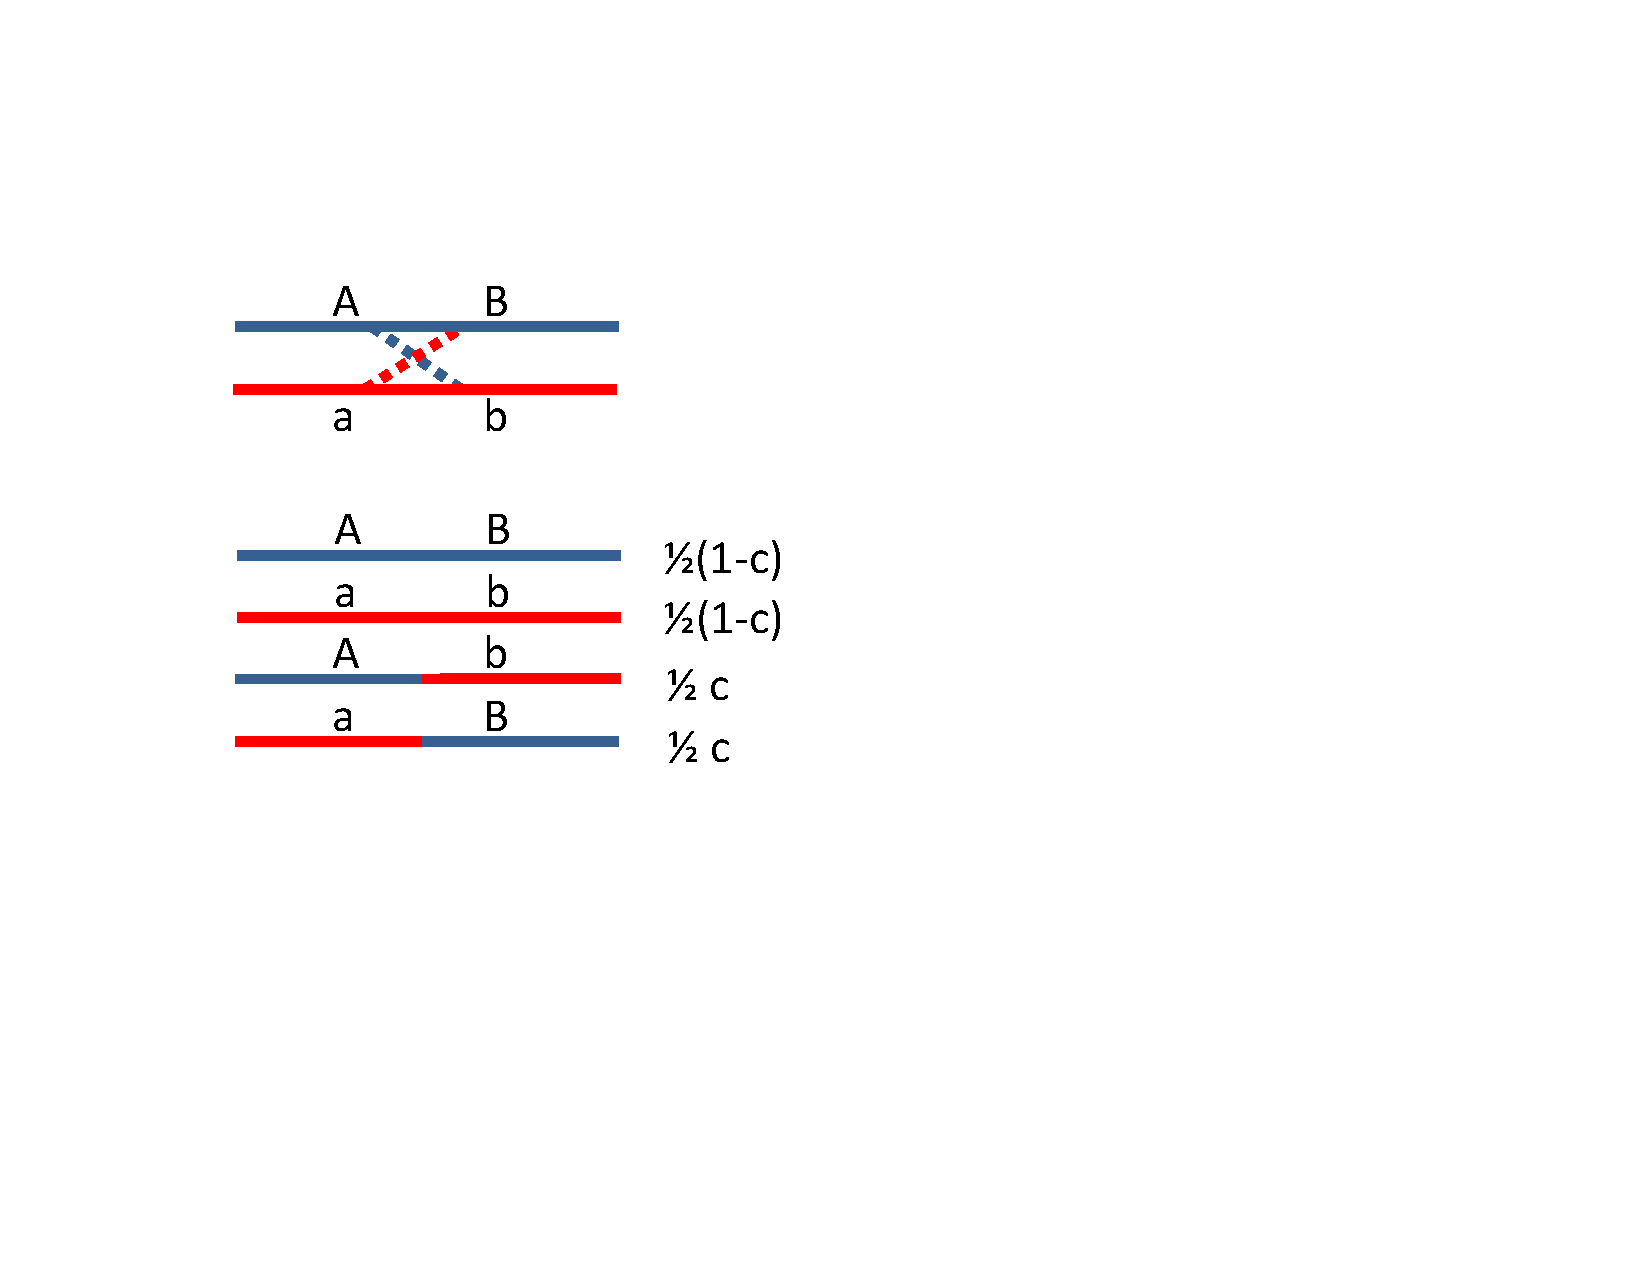
\includegraphics[width= 0.8 \textwidth ]{figures/LD_decay/recom_cartoon.pdf}
\end{center}
\caption{A cartoon of the possible outcomes of meiosis. The blue and
  red lines are two copies of a chromosome in an  individual who is
  heterozygote for a AB and an ab haplotype. The dotted lines show a
  possible crossover between the two chromosomes. The four possible
  outcomes of meiosis are show below, the probablity of each is given
  to the right (assuming
  a recombination fraction of $c$ between the two loci).} \label{fig:recom_cartoon}
\end{marginfigure}


\paragraph{Recombination}
To understand correlations between loci we need to
understand recombination a bit more carefully. Let us consider a heterozygous individual, containing $AB$ and $ab$ haplotypes.
If no recombination occurs between our two loci in this individual, then these
two haplotypes will be transmitted intact to the next generation. While if a
recombination (i.e. an odd number of crossing over events) occurs between the
two parental haplotypes, then $\nicefrac{1}{2}$ the time the child receives an
$Ab$ haplotype and $\nicefrac{1}{2}$ the time the child receives an $aB$
haplotype. See Figure \ref{fig:recom_cartoon}. Effectively, recombination breaks up the association between loci.
For linked markers we'll define the recombination fraction ($x$) to be the probability
of an odd number of crossing over events between our loci in a single
meiosis. The recombination fraction between a pair of loci can range from $0$ to
$\nicefrac{1}{2}$, with $c=\nicefrac{1}{2}$ corresponding markers far
enough apart on a chromosome that many recombination events occur
between them (loci on different automosomes also have a $c=\nicefrac{1}{2}$).  In practice we'll often be
interested in relatively short regions such that recombination is relatively
rare, and so we might think that $c=c_{BP}L \ll \frac{1}{2}$, where $c_{BP}$ is the
average recombination rate (in Morgans) per base pair (typically $\sim 10^{-8}$ ) and L is
the number of base pairs separating our two loci.\\
%JRI: I think you'd be better to stick with A_1A_2 and B_1B_2 notation rather than AaBb. Ideally be consistent with this throughout the book, maybe with a sidenote the first time you do it saying something like "I use A_1A_2 but you will often see Aa. I do it this way as to avoid confusion about perceived dominance or ancestral state."

\paragraph{Linkage disequilibrium}
The (horrible) phrase linkage
disequilibrium (LD) refers to the statistical non-independence
(i.e. a correlation)  of
alleles in a population at different loci \citep{lewontin1960evolutionary,slatkin2008linkage}. It's a fantastically useful concept; LD is key to our understanding of diverse topics, from sexual selection and speciation to the limits of genome-wide association studies.

Our two biallelic loci, which segregate alleles $A/a$ and $B/b$, have allele
frequencies of $p_A$ and $p_B$ respectively. The frequency of the two locus haplotype AB is $p_{AB}$,
and likewise for our other three combinations. If our loci were
statistically independent then $p_{AB} = p_Ap_B$, otherwise $p_{AB} \neq p_Ap_B$
We can define a covariance between the $A$ and $B$ alleles at our two
loci\sidenote{Here again we are making use of a covariance of discrete
random variables, see Appendix \eqn \eqref{eqn:binary_covar}, where the
first variable is drawing haplotype with an $A$ at the first locus,
and the second is drawing a B allele at the other locus.} as
%JRI: sure, but a few lines above you define LD as a correlation so
%why are you shis owing us a covariance?
\begin{equation}
D_{AB} = p_{AB} - p_Ap_B  \label{eqn:LD_def}
\end{equation}
and likewise for our other combinations at our two loci
($D_{Ab},~D_{aB},~D_{ab}$).
Gametes with two similar case alleles (e.g. A and B, or a and b) are known as \emph{coupling} gametes, and those with different case alleles are known as \emph{repulsion} gametes (e.g. a and B, or A and b). Then, we can think of $D$ as measuring the \emph{excess} of coupling to repulsion gametes.
These $D$ statistics are all closely
related to each other as $D_{AB} = - D_{Ab}$ and so on. Thus we only
need to specify one $D_{AB}$ to know them all, so we'll drop the
subscript and just refer to $D$. Also a handy result is that we can rewrite our haplotype
frequency $p_{AB}$ as
\begin{equation}
p_{AB} = p_Ap_B+D. \label{eqn:ABviaD}
\end{equation}
If $D=0$ we'll say the two loci are in linkage equilibrium, while if
$D>0$ or $D<0$ we'll say that the loci are in linkage
disequilibrium (we'll perhaps want to test whether $D$ is
statistically different from $0$ before making this choice). Linkage
disequilibrium is a horrible phrase, as it risks muddling the concepts
of genetic linkage and linkage disequilibrium. Genetic linkage refers to the
linkage of multiple loci due to the fact that they
are transmitted through meiosis together (most often because the
loci are on the same chromosome). Linkage disequilibrium merely refers
to the covariance between the alleles at different loci; this may in
part be due to the genetic linkage of these loci but does not
necessarily imply this (e.g. genetically unlinked loci can be in LD
due to population structure). \\
%JRI: good explanation. at beginning of section you say LD is a horrible term but don't explain. tempted to move that comment here or move this explanation there, as otherwise it seems odd and alone

\begin{question}{}
You genotype 2 bi-allelic loci (A \& B) segregating in two mouse subspecies (1 \& 2) which mate randomly among themselves, but have not historically interbreed since they speciated. The frequencies of haplotypes in each population are:
\begin{center}
\begin{tabular}{|c|cccc|}
\hline
Pop    & $p_{AB}$    & $p_{Ab}$ &    $p_{aB}$ &    $p_{ab}$\\
\hline
1 &    .02    & .18 &     .08 &    .72\\
2&    .72 &    .18 &    .08 &    .02\\
\hline
\end{tabular}
\end{center}

{\bf A)} How much LD is there within species? (i.e. estimate D)\\

{\bf B)} If we mixed individuals from the two species together in equal proportions, we could form a new population with $p_{AB}$ equal to the average frequency of $p_{AB}$ across species 1 and 2. What value would D take in this new population before any mating has had the chance to occur? \\
\end{question}



\begin{figure}
\begin{center}
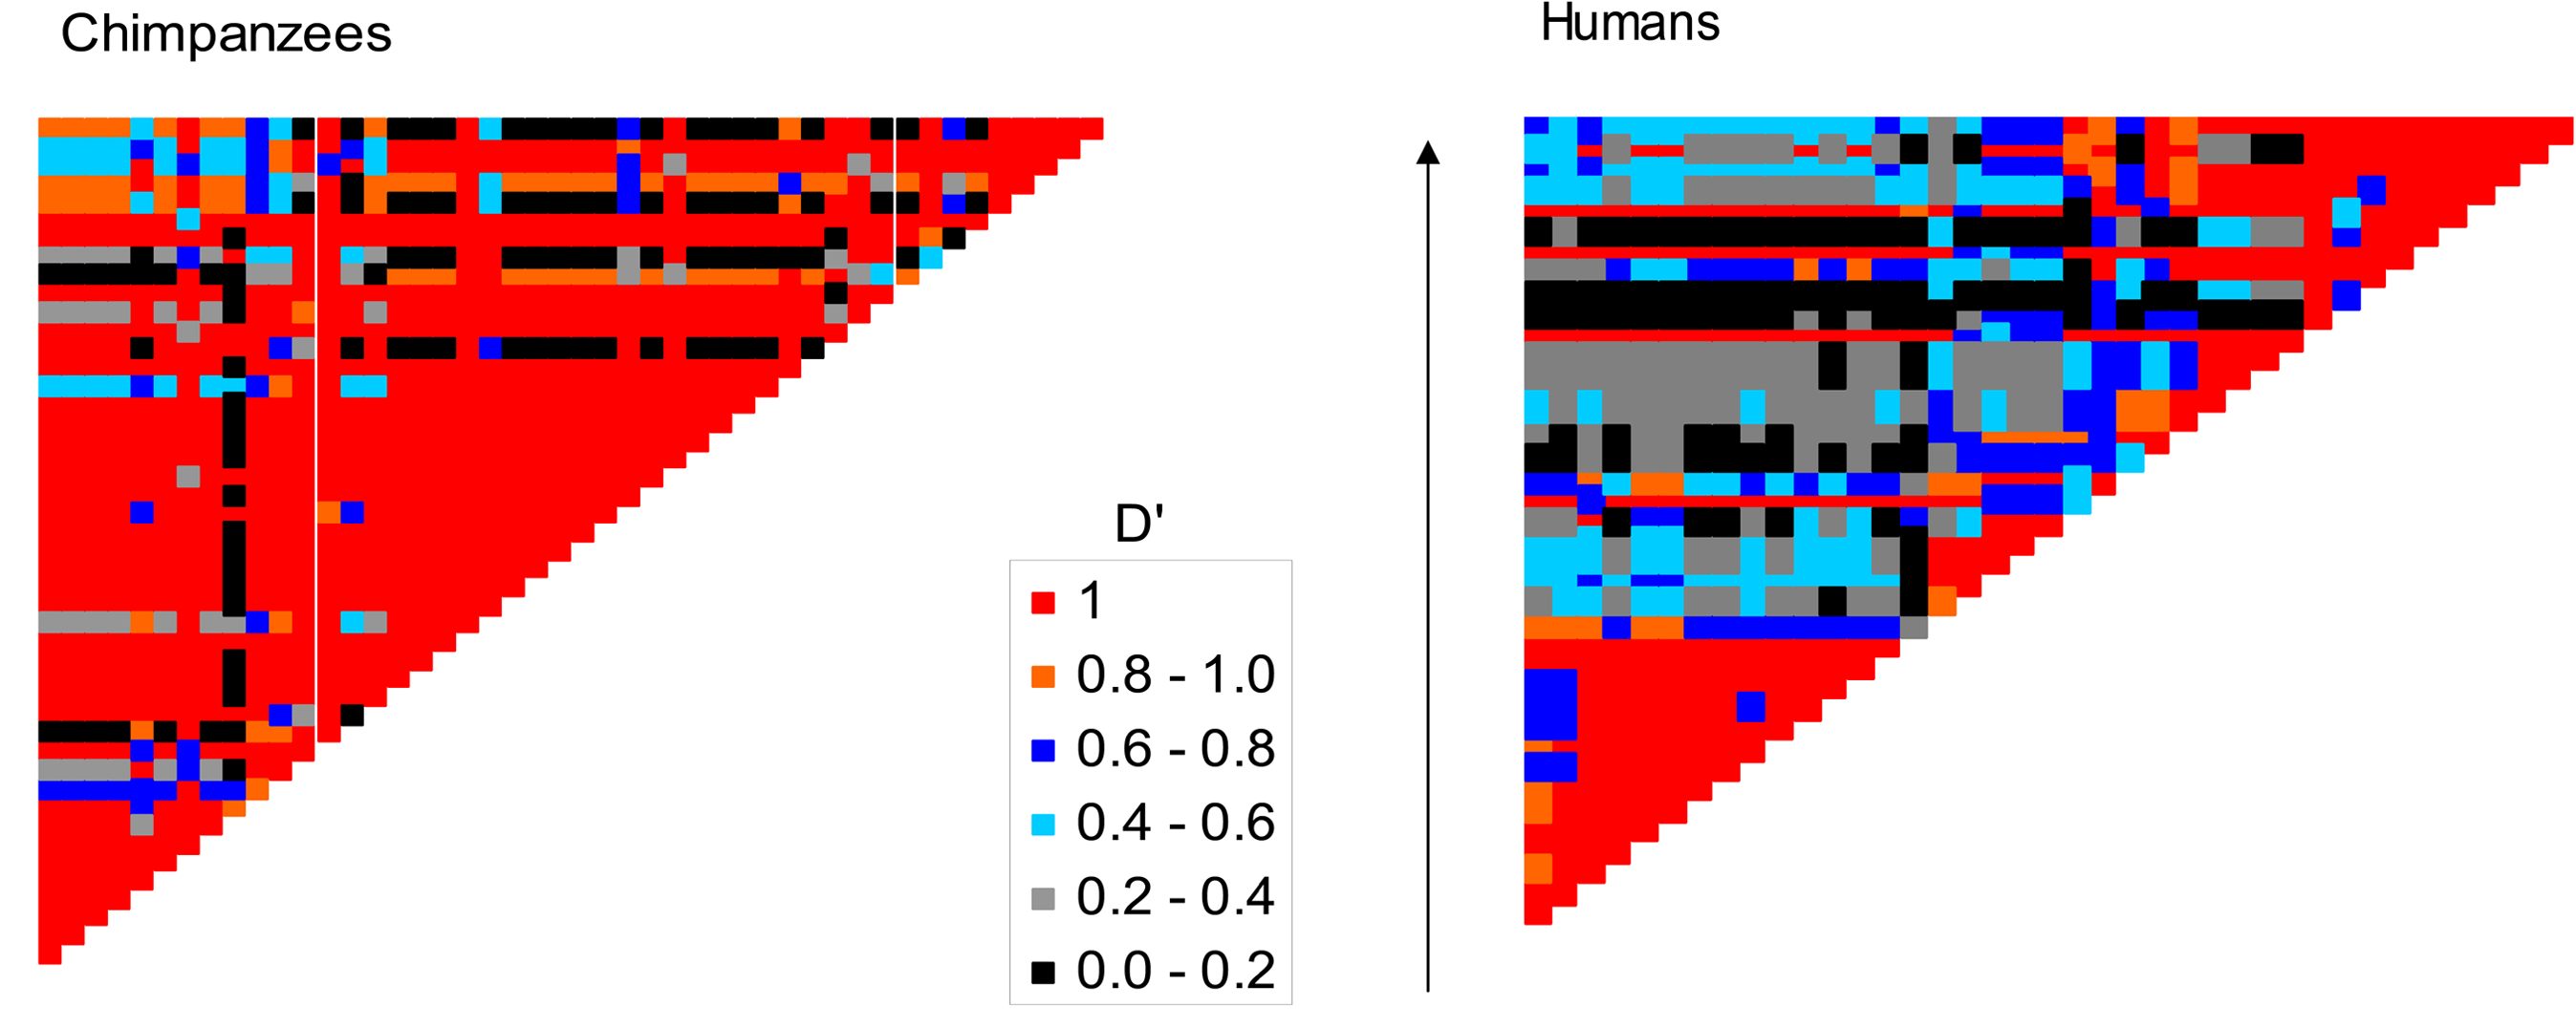
\includegraphics[width= 0.8 \textwidth ]{Journal_figs/alleles_genotypes/TAPS_hotspot/Taps_hotspot.png}
\end{center}
\caption{LD across the TAP2 gene region in a sample of Humans and
  Chimps, from \citet{ptak2004absence}, \PLOSccBY. The rows and columns are consecutive SNPs, with each cell giving
  the absolute $D^{\prime}$ value between a pair of SNPs. Note that these
are different sets of SNPs in the two species, as shared polymorphisms
are very rare.} \label{fig:TAPS_hotspot}
\end{figure}

Our linkage  disequilibrium statistic $D$ depends strongly on the
allele frequencies of the two loci involved. One common way to
partially remove this dependence, and make it more comparable across
loci, is to divide $D$ through by its  maximum possible value given
the frequency of the loci. This normalized statistic is called
$D^{\prime}$ and varies between $+1$ and $-1$. In Figure
\ref{fig:TAPS_hotspot} there's an example of LD across the TAP2 region
in human and chimp. Notice how physically close SNPs, i.e. those close
to the diagonal, have higher absolute values of $D^{\prime}$ as
closely linked alleles are separated by recombination less often
allowing high levels of LD to accumulate. Over large physical
distances, away from the diagonal, there is lower $D^{\prime}$. This is
especially notable in humans as there is an intense, human-specific recombination
hotspot in this region, which is breaking down LD between opposite
sides of this region.

Another common statistic for summarizing LD is $r^2$ which we write as
\begin{equation}
r^2 = \frac{D^2}{p_A(1-p_A) p_B(1-p_B) }
\end{equation}
As $D$ is a covariance, and $p_A(1-p_A) $ is the variance of an allele
drawn at random from locus $A$, $r^2$ is the squared correlation
coefficient.\sidenote{See Appendix \eqn \eqref{eqn:def_corr} for the
  definition of a correlation coefficient.} \\ %Note that this $r$ in $r^2$ is NOT the recombination
fraction.   \\

\begin{marginfigure}
\begin{center}
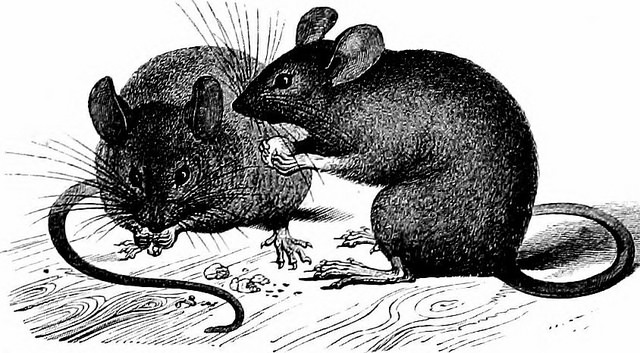
\includegraphics[width=\textwidth]{illustration_images/alleles_genotypes/Mus_musculus/20746324002_e014b4fcc6_z.jpg}
\end{center}
\caption{{\it Mus musculus}. \BHLNKC{A history of British quadrupeds, including the Cetacea. 1874. Bell T., Tomes, R. F.m Alston E. R.}{https://www.flickr.com/photos/internetarchivebookimages/20746324002/in/photolist-x4m4C7-v8ZA8q-x5EdgX-w8gFve-x57DCB-v8ZCQE-xBhkkq-vdFPLY-x2JeQJ-x5WJ8J-tG8BSM}{Cornell University Library}} \label{fig:Mouse}
\end{marginfigure}


Figure \ref{fig:Mouse_LD} shows $r^2$ for pairs of SNPs at
various physical distances in two population samples of {\it Mus musculus
  domesticus}. Again LD is highest between physically close markers as LD is being generated faster than it can
decay via recombination; more distant markers have much lower LD as
here recombination is winning out. Note the decay of LD is much
slower in the advanced-generation cross population than in the natural wild-caught population. This persistence of LD across megabases is due to the limited number of generations for recombination
since the cross was created.


\begin{figure}
\begin{center}
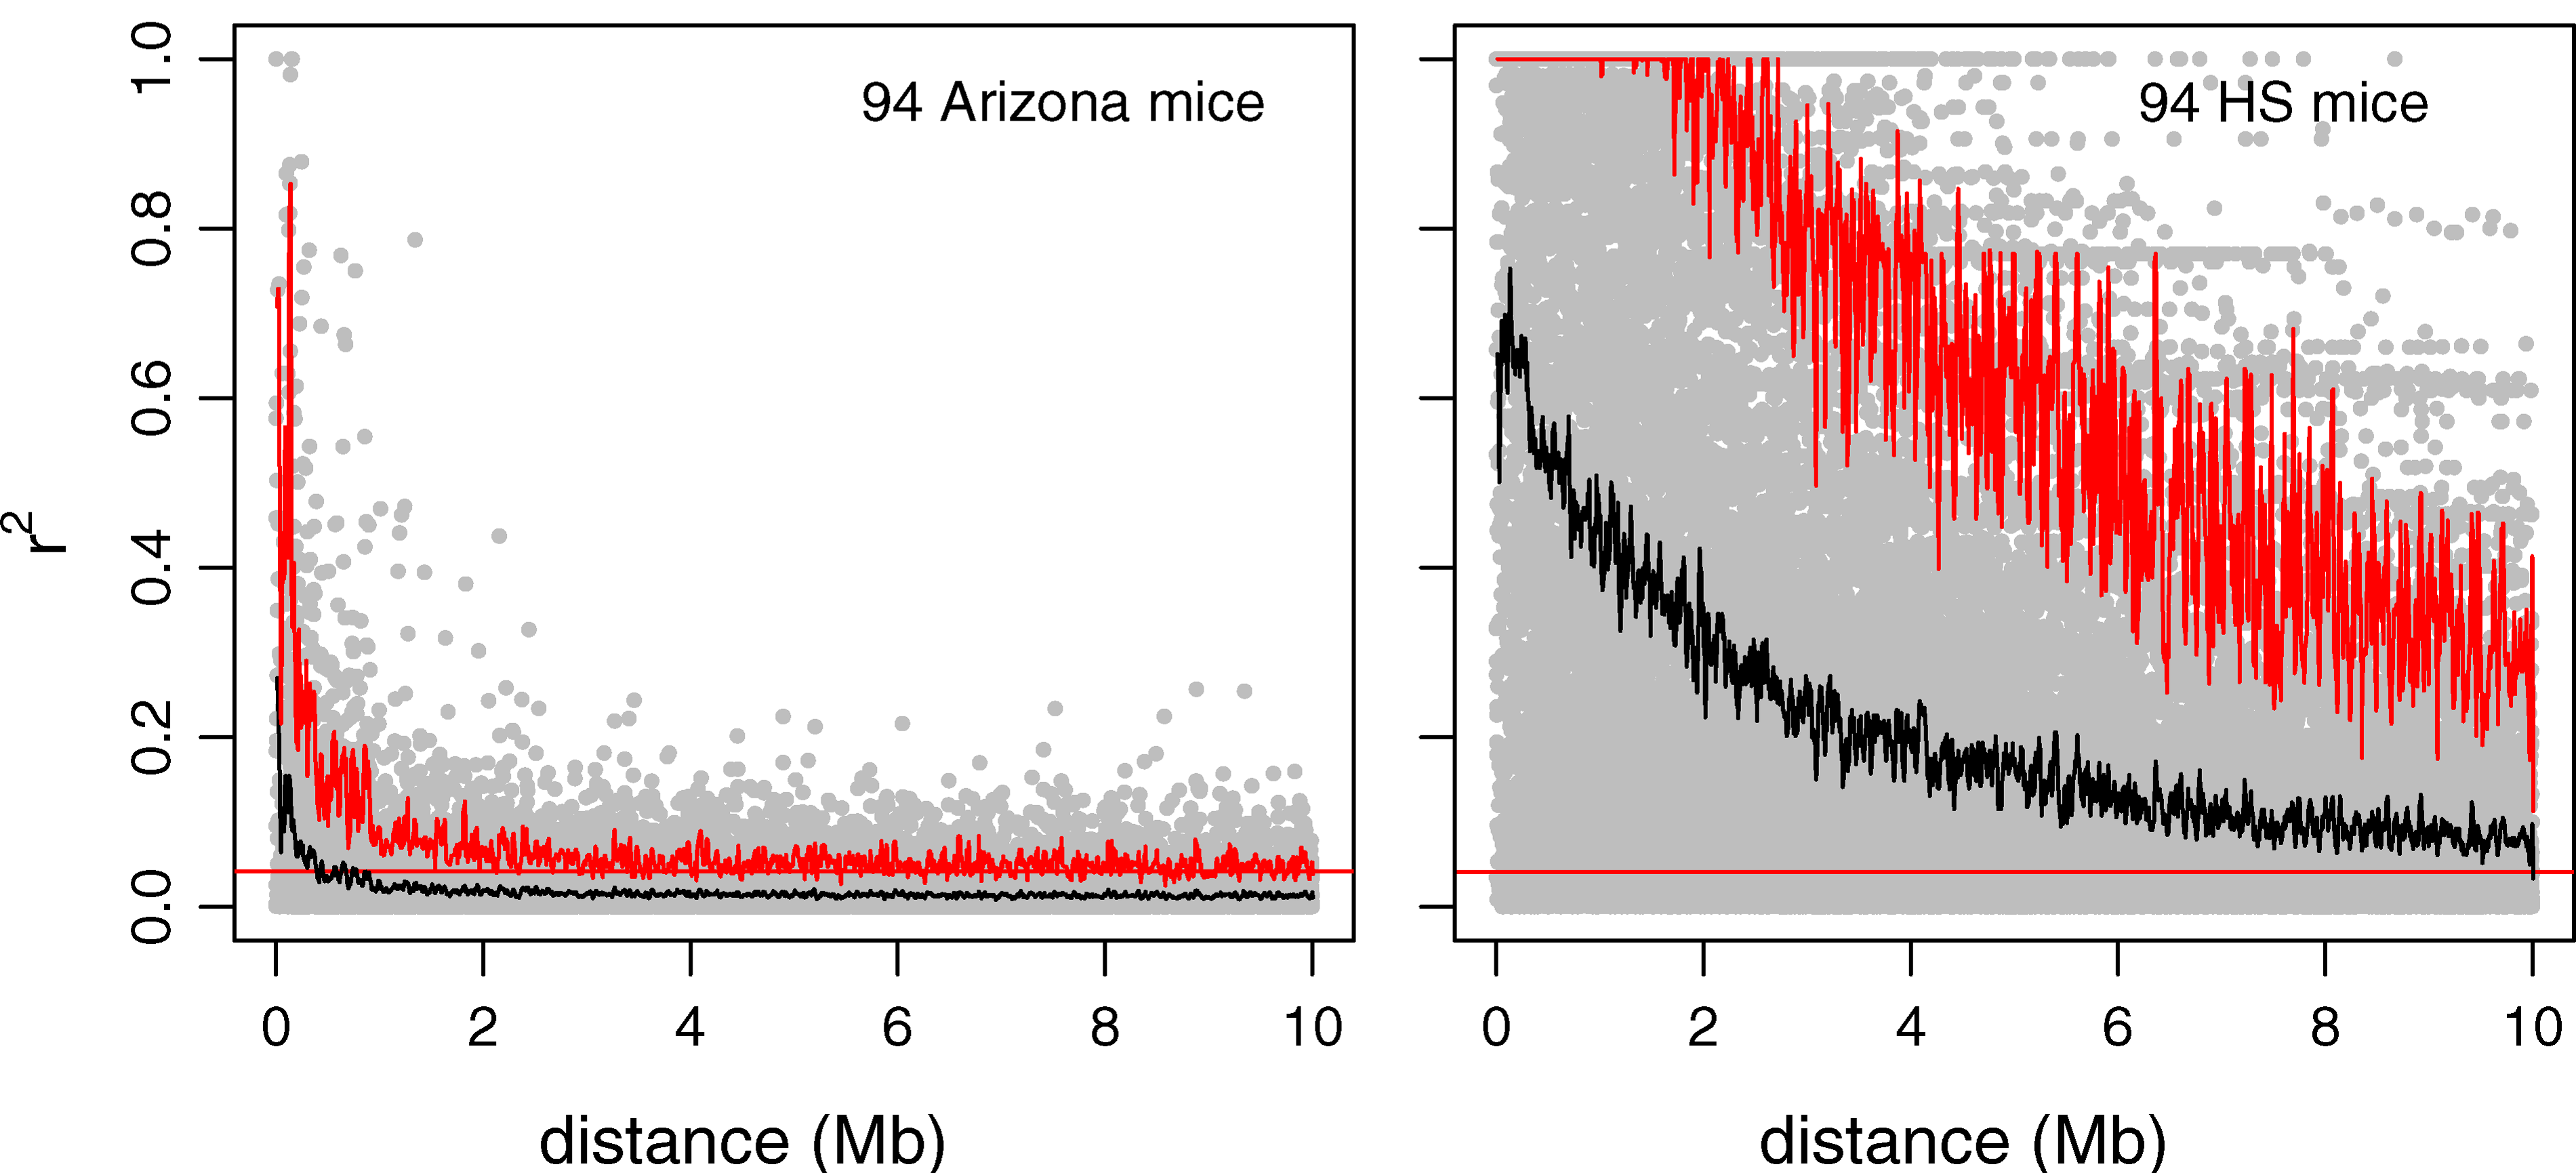
\includegraphics[width=0.8 \textwidth]{Journal_figs/alleles_genotypes/mouse_LD/mouse_LD_Laurie_et_al.png}
\end{center}
\caption{The decay of LD for autosomal SNPin {\it Mus musculus
  domesticus}, as measured by $r^2$, in a wild-caught mouse population
  from Arizona and a set of advanced-generation crosses between inbred lines of lab mice. Each dot gives the $r^2$ for a
  pair of SNPs a given physical distance apart, for a total of $\sim
  3000$ SNPs. The solid black line gives the mean, the jagged red line the
  $95^{th}$ percentile, and the flat red line a cutoff for
  significant $LD$. From \citet{Laurie:07}, \PLOSccBY. } \label{fig:Mouse_LD}
\end{figure}
%JRI: what's "HS" in the figure on the right?


\paragraph{The generation of LD.}
Various population genetic forces can generate LD \citep{slatkin2008linkage}. Selection can generate LD by favouring particular combinations of
alleles. Genetic drift will also generate LD, not because particular
combinations of alleles are favoured, but simply because at random particular
haplotypes can by chance drift up in frequency. Mixing between
divergent populations can also generate LD \citep{nei1973linkage}, as we saw in the mouse
question above.
%JRI: super weird not to mention mutation as generating LD

\paragraph{The decay of LD due to recombination}

We will now examine what happens to LD over the generations if, in a very large population  (i.e. no genetic drift and frequencies of our loci thus follow their expectations), we
only allow recombination to occur. 
To do so, consider the frequency of our $AB$ haplotype in the next generation,
$p_{AB}^{\prime}$. We lose a fraction $c$ of our $AB$ haplotypes to
recombination ripping our alleles apart but gain a fraction $cp_A p_B$ per generation from other
haplotypes recombining together to form $AB$ haplotypes. Thus in the
next generation
\begin{equation}
p_{AB}^{\prime} = (1-c)p_{AB} + cp_Ap_B \label{new_hap_freq}
\end{equation}
The last term above, in \eqn \ref{new_hap_freq}, is $c(p_{AB}+p_{Ab})(p_{AB}+p_{aB})$ simplified, which is the probability of recombination in the different diploid genotypes that
could generate a $p_{AB}$ haplotype. \\

We can then write the change in the frequency of the $p_{AB}$
haplotype as
\begin{equation}
\Delta p_{AB} = p_{AB}^{\prime} -p_{AB} = -c p_{AB} + cp_Ap_B = - c D
\end{equation}
\begin{marginfigure}
\begin{center}
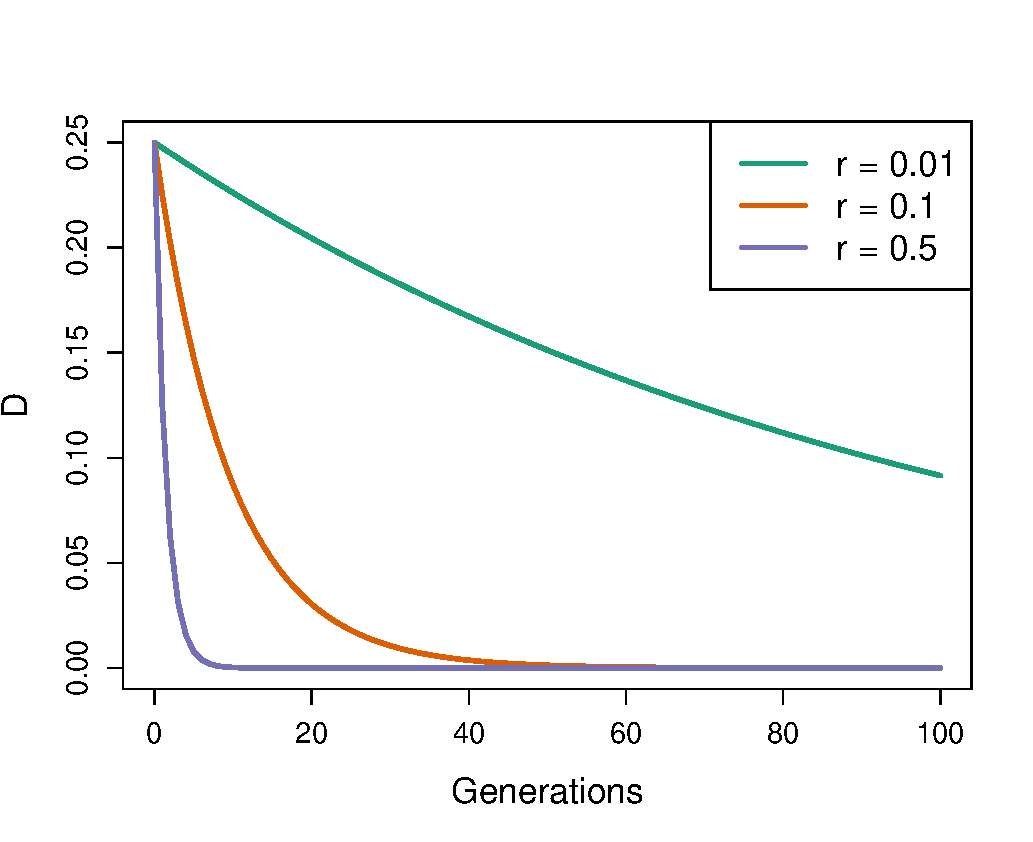
\includegraphics[width=\textwidth]{figures/LD_decay/LD_decay_time.pdf}  %https://github.com/cooplab/popgen-notes/blob/master/Rcode/LD/LD_decay.R
\end{center}
\caption{The decay of LD from an initial value of $D_0=0.25$ over time
  (Generations) for a pair of loci a recombination fraction $c$
  apart. \gitcode{https://github.com/cooplab/popgen-notes/blob/master/Rcode/LD/LD_decay.R}}\label{fig:LD_time}
\end{marginfigure}
\begin{marginfigure}
\begin{center}
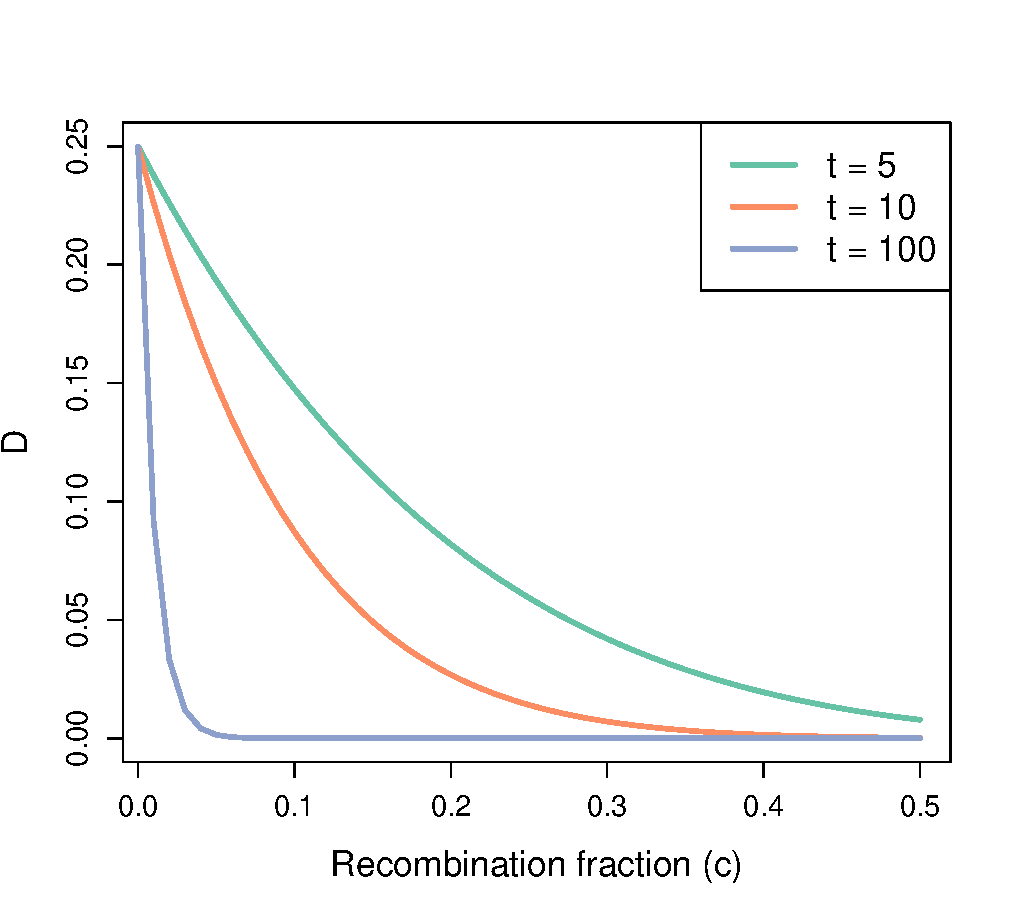
\includegraphics[width=\textwidth]{figures/LD_decay/LD_decay_recom.pdf}
\end{center}
\caption{The decay of LD from an initial value of $D_0=0.25$ due to recombination over $t$ generations, plotted across possible recombination fractions ($c$) between our pair of loci. \gitcode{https://github.com/cooplab/popgen-notes/blob/master/Rcode/LD/LD_decay.R}} \label{fig:LD_recom}
\end{marginfigure}
%JRI: shouldn't y-axis labels for both be \Delta D?
So recombination will cause a decrease in the frequency of $p_{AB}$ if
there is an excess of $AB$ haplotypes within the population ($D>0$), and an
increase if there is a deficit of $AB$ haplotypes within the
population ($D<0$). Our LD in the next generation is
\begin{align}
D^{\prime} & = p_{AB}^{\prime} - p'_{A}p'_{B} \nonumber\\
& = (p_{AB} + \Delta p_{AB}) - (p_{A} + \Delta p_{A})(p_{B} + \Delta p_{B}) \nonumber\\
& = p_{AB} + \Delta p_{AB} - p_{A}p_{B} \nonumber\\
& = (1-c) D
\end{align}
where we can cancel out $\Delta p_{A}$ and $\Delta p_{B}$ above because recombination only changes haplotype, not allele, frequencies.
So if the level of LD in generation $0$ is $D_0$, the level $t$
generations later ($D_t$) is
\begin{equation}
D_t=  (1-c)^t D_0
\end{equation}
Recombination is acting to decrease LD, and it does so
geometrically at a rate given by $(1-c)$ \citep{weinberg1909vererbungsgesetze,jennings1917numerical}. If $c \ll 1$ then we can
approximate this by an exponential and say that
\begin{equation}
D_t \approx  D_0 e^{-ct}  \label{eqn_LD_decay}
\end{equation}\\

%{\bf Q}\arabic{Question} \refstepcounter{Question}
\begin{question}{}
You find a hybrid population between the two mouse subspecies
described in the question above, which appears to be comprised of
equal proportions ($50/50$) of ancestry from the two subspecies.  You estimate LD between the two markers to be $D=0.0723$. On the basis of previous work you estimate that the two loci are separated by a recombination fraction of 0.1. Assuming that this hybrid population is large and was formed by a single mixture event, can you estimate how long ago this population formed? \\
\end{question}
%JRI: assumes r from previous problem. would be clearer to mention this or give r. also just says "LD" but should be more specific that you mean D.
\begin{marginfigure}[2cm]
\begin{center}
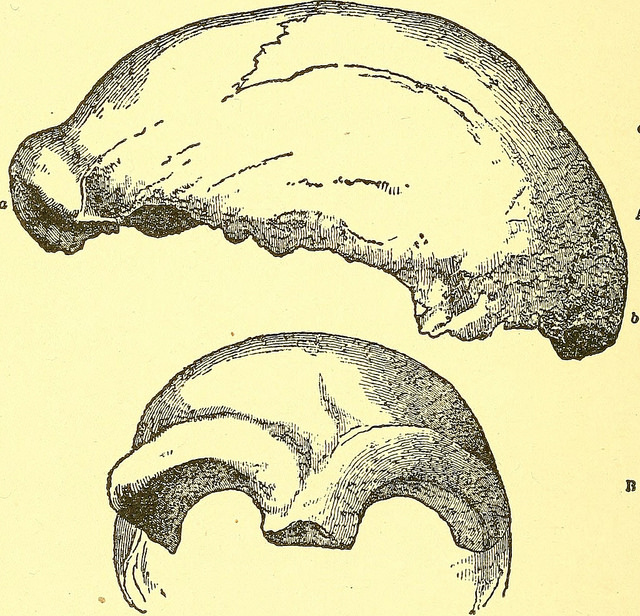
\includegraphics[width=\textwidth]{illustration_images/alleles_genotypes/Neanderthal/14800262343_f21929987a_z.jpg}
\end{center}
\caption{The earliest discovered fossil of a Neanderthal, fragments of a skull found in a cave in the Neander Valley in Germany. \IANC{Man's place in nature. 1890. Huxley, T. H.}{https://archive.org/stream/mansplaceinnatur02huxl/mansplaceinnatur02huxl\#page/154/mode/1up}{The Library of Congress}} \label{fig:Neand_skull}
\end{marginfigure}

A particularly striking example of the decay of LD generated by
the mixing of populations is offered by the LD created by the
interbreeding between humans and Neanderthals \citep{Sankararaman:12}. Neanderthals and modern
humans diverged from each other likely over half a million years ago,
allowing time for allele frequency differences to accumulate between
the Neanderthal and modern human populations. The two populations spread back into secondary contact when
humans moved out of Africa over the past hundred thousand years or
so. One of the most exciting findings from the sequencing of the
Neanderthal genome was that modern-day people with Eurasian ancestry
carry a few percent of their genome derived from the Neanderthal
genome, via interbreeding during this secondary contact \citep{green2010draft}. To date the timing of this
interbreeding, \citet{Sankararaman:12} looked at the LD in modern
humans between pairs of alleles found to be derived from the Neanderthal
genome (and nearly absent from African populations).
In Figure \ref{fig:LD_Neanderthal} we show the average LD between these loci as a function of the genetic distance ($c$) between them, from
the work of
\citeauthor{Sankararaman:12}.
\begin{figure}
\begin{center}
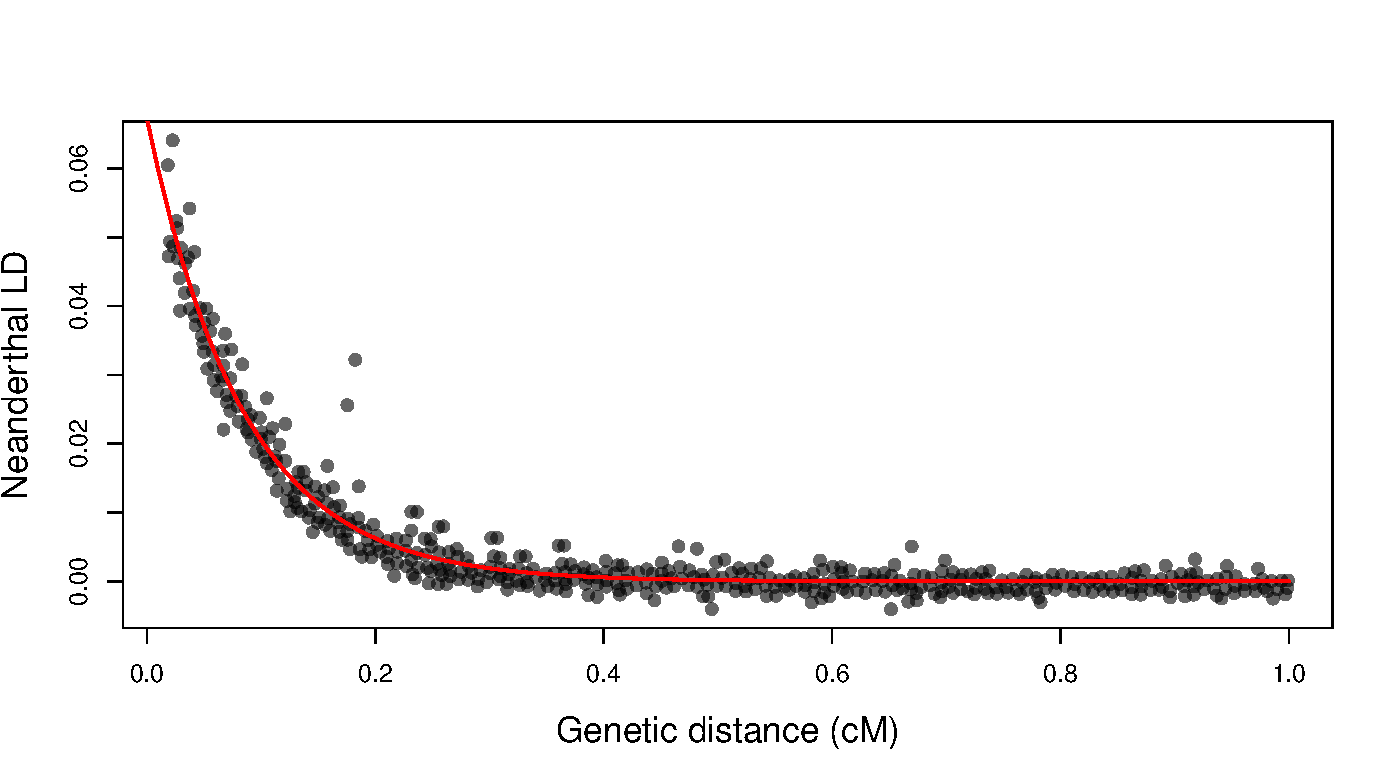
\includegraphics[width=0.8 \textwidth]{Journal_figs/alleles_genotypes/Neanderthal_LD/European_neanderthal_LD.pdf}
\end{center}
\caption{The LD between putative-Neanderthal alleles in a modern European population (the CEU sample from the 1000 Genomes Project). Each point represents the average D statistic between a pair of alleles at loci at a given genetic distance apart (as given on the x-axis and measured in centiMorgans (cM)). The putative Neanderthal alleles are alleles where the Neanderthal genome has a derived allele that is at very low frequency in a modern-human  West African population sample (thought to have little admixture from Neanderthals). The red line is the fit of an exponential decay of LD, using non-linear least squared (nls in R).}
\label{fig:LD_Neanderthal}
\end{figure}

Assuming a recombination rate $r$, we can fit the exponential decay of LD predicted by \eqn \eqref{eqn_LD_decay} to the data points in this figure;
the fit is shown as a red line. Doing this we estimate $t=1200$
generations, or about 35 thousand years (using a human generation time of 29
years). Thus the LD in modern Eurasians, between alleles derived from
the interbreeding with Neanderthals, represents over thirty thousand years of
recombination slowly breaking down these old
associations. \sidenote{The calculation done by
  \citet{Sankararaman:12} is actually a bit more involved as they
account for inhomogeneity in recombination rates and arrive at a date
of  47,334 -- 63,146 years.}
%JRI: /marginnote with no number used well for definitions. /sidenote should be used for comments about specific parts of the text
